%----------------------------------------------------------
% MAVIS final project report (ESE template, 25-40 pages)
% Build: python3 build.py && pdflatex report.tex (twice)
%----------------------------------------------------------
\documentclass[12pt,singleside,a4paper]{article}
\usepackage{epsfig}
\usepackage{cite}
\usepackage{geometry}
\geometry{left=20mm,right=20mm,top=20mm,bottom=50mm}
\usepackage{graphicx}
\usepackage{amsmath,amssymb}
\usepackage{array,booktabs,tabularx,longtable,multirow}
\usepackage{float}
\usepackage{subcaption}
\usepackage{enumitem}
\usepackage{xcolor}
\usepackage{pifont}
\usepackage{tikz}
\usetikzlibrary{arrows.meta,positioning,shapes.geometric,fit,calc,backgrounds}
\usepackage{microtype}
\usepackage[hidelinks]{hyperref}
\graphicspath{{figures/}{./}}
\setlength{\emergencystretch}{3em}
\renewcommand{\arraystretch}{1.2}
\newcommand{\cmark}{\ding{51}}
\newcommand{\xmark}{\ding{55}}
% \tbd{...} marks a value the team still has to fill in (printed in red).
\newcommand{\tbd}[1]{\textcolor{red}{[#1]}}
\definecolor{mbrand}{HTML}{7C6CFF}
\definecolor{mbsoft}{HTML}{ECEAFF}
\pagestyle{plain}
\setcounter{tocdepth}{2}
\begin{document}
\pagenumbering{arabic}
\begin{titlepage}
\vspace*{0.025cm}
{\centering
\mbox{}\\
{\Large\textbf {MAVIS: Multimodal Assistance for\\ Vision, Interaction, and Speech}}\\[0.3cm]
{\large A Gesture-Controlled System for Document Question\\ Answering, Live English--Hindi Speech Translation\\ and Scene Assistance}\\
\vspace{0.55cm}
submitted in partial fulfillment of the requirement\\
for the award of the Degree of\\\vspace{0.65cm}
{\large\textbf {Bachelor of Technology}}\\
in \\
{\large\textbf {Computer Science and Engineering}}\\
\vspace{0.50cm}
by\\
\vspace{0.55cm}
{\large \textbf {Varad Chipkar (2023800011)}}\\
{\large \textbf {Yogita Aher (2023800003)}}\\
{\large \textbf {Harshvardhan Singh Deora (2023800015)}}\\
\vspace{0.55cm} 
under the guidance of\\ 
\vspace{0.55cm}
\hspace{.05cm} {\large \textbf {Prof. Suhas Kakade}}\\
\begin{figure}[h]
\centering

\includegraphics[scale=0.7]{spitlogo.pdf}
\end{figure}
\hspace{.05cm}
\hspace{.05cm}
\textbf{Department of Computer Science and Engineering}\\
Bharatiya  Vidya Bhavan's\\
Sardar Patel Institute of Technology\\
(Autonomous Institute Affiliated to University of Mumbai)\\
Munshi Nagar, Andheri-West, Mumbai-400058\\
University of Mumbai\\
2026-2027}
\end{titlepage}
\newpage
\thispagestyle{empty}
\vspace*{0.2cm}
\vspace{1cm}
\begin{center}
 \large\textbf{Approval Certificate}
\end{center}
\vspace{2cm}
This is to certify that the Project entitled ``MAVIS (Multimodal Assistance for Vision, Interaction, and Speech): A Gesture-Controlled System for Document Question Answering, Live English--Hindi Speech Translation and Scene Assistance'' by Varad Chipkar, Yogita Aher and Harshvardhan Singh Deora is approved  for the partial fulfillment of Major Project - I for the Final Year Project towards obtaining the Degree of Bachelor of Technology in Computer Science and Engineering from University of Mumbai.\\
\\
\\
\\
\\
\\
\textbf{Project Guide} \hspace{3.5in} \textbf{External Examiner}\\ 
\\
\\
\\
\\
\textbf {(signature)} \hspace{3.75in} \textbf{(signature)} \\
\\
\vspace{1cm}
\textbf {Name:} Prof.\ Suhas Kakade \hspace{2.3in} \textbf{Name:}\\ 
\vspace{1cm}
\textbf {Date:} \hspace{4.2in} \textbf{Date:}\\ 
\vspace{1cm}
\\
\\
\textbf {Head of Department} \hspace{3in} \textbf{Principal}\\ 
\vspace{2cm}
\begin{center}
\textbf{Seal of the Institute}\\
\end{center}


\section*{\centering{Declaration}}

\vspace{3.5cm}
We wish to state that the work embodied in this work titled ``MAVIS (Multimodal Assistance for Vision, Interaction, and Speech): A Gesture-Controlled System for Document Question Answering, Live English--Hindi Speech Translation and Scene Assistance'' forms our own contribution to the work carried out under the guidance of Prof.\ Suhas Kakade at the Sardar Patel Institute of Technology. We declare that this written submission represents our ideas in our own words and where others' ideas or words have been included, we have adequately cited and referenced the original sources. We also declare that we have adhered to all principles of academic honesty and integrity and have not misrepresented or fabricated or falsified any idea/data/fact/source in our submission.
\\
\\
\\
\noindent\begin{tabular*}{\textwidth}{@{}l@{\extracolsep{\fill}}cr@{}}
\textbf{Varad Chipkar} & \textbf{Yogita Aher} & \textbf{Harshvardhan Singh Deora}\\[4cm]
\textbf{2023800011} & \textbf{2023800003} & \textbf{2023800015}\\
\end{tabular*}
\vspace{1cm}

\pagebreak
\section*{Abstract}
\addcontentsline{toc}{section}{Abstract}
People who cannot easily read print, follow a spoken language or see their surroundings usually need a separate application for each of these needs, each with its own controls. This project builds \textbf{MAVIS} (Multimodal Assistance for Vision, Interaction, and Speech), a single system in which the user's \emph{hand} chooses the assistance. MAVIS joins four independently developed components: (1)~a \textbf{gesture recognition} module (MediaPipe Hands with a palm-frame, rule-based classifier and a temporal stabiliser) that acts as the controller of the whole product; (2)~an \textbf{OCR + LLM} document assistant that captures printed pages from a camera, reads them with RapidOCR PP-OCRv5 and answers questions with a local Gemma~3 4B model, citing the page and an exact quote that is checked against the scanned text; (3)~a \textbf{live English-to-Hindi speech translation} module built on streaming Whisper recognition with LocalAgreement-2 commitment, MT3-C scheduled opus-mt drafts and NLLB-200 final translations, shown as film-style subtitles over the live camera picture; and (4)~\textbf{Drishti}, a local-first scene assistant for blind and visually impaired users with eleven camera modes, deterministic hazard scoring and voice control in English and eight Indian languages.

A thumbs-up arms the controller; one, two or three fingers within eight seconds open OCR + LLM, Live Translation or Drishti respectively, and the chosen module starts working on its own; an open palm turns it off. A Python hub serves all modules from one launcher on one laptop, runs the translation package in its own environment and process, assigns the laptop's camera and microphone to every module (the OCR module can alternatively stream from the DroidCam phone app over Wi-Fi), gives the whole product one colour scheme, and starts with a single \texttt{run.bat}. No component's source code was modified: 314 original files are byte-identical against a SHA-256 manifest. The original test suites pass (gesture 112; OCR 149 passed, 5 skipped; translation 120 passed, 3 skipped) along with 21 new integration tests. In the end-to-end test with real hand photographs the controller went from idle to an auto-started Drishti in under 6\,s at 13.1\,ms mean server time per frame; on the demonstration laptop the translation models loaded in 13.4\,s and produced Hindi subtitles from live speech.

\vspace{0.3cm}
\noindent\textbf{Keywords:} gesture-controlled interface, assistive technology, MediaPipe, OCR, grounded question answering, streaming speech translation, Whisper, NLLB-200, local-first AI, system integration.
\pagebreak
\listoffigures
\addcontentsline{toc}{section}{List of Figures}
\vspace{1em}
\listoftables
\addcontentsline{toc}{section}{List of Tables}
\pagebreak
{\footnotesize\setlength{\parskip}{0pt}\linespread{0.92}\selectfont\tableofcontents}
\pagebreak

%=====================================================================
\section{Introduction}
The World Health Organization estimates that at least 2.2 billion people live with a near or distance vision impairment \cite{who2019}, with a large share of that burden in South Asia \cite{bourne2017}. India is also strongly multilingual: much spoken and written information reaches people in a language that is not their first. Smartphones and laptops already carry the sensors needed to help---a camera and a microphone---and commercial applications such as Seeing AI \cite{seeingai} and Be My Eyes \cite{bemyeyes} show what a camera and a speech interface can do. Each underlying capability has also become practical on ordinary hardware: real-time hand tracking \cite{zhang2020mediapipe}, CPU-friendly OCR \cite{du2020ppocr}, small language and vision-language models \cite{gemma3,marafioti2025}, and streaming speech recognition and translation \cite{radford2023,machacek2023,nllb2022}.

What is still missing is a product that brings these capabilities together behind one simple control. Each member of our team had built one part of the problem, and each part worked on its own:
\begin{itemize}[leftmargin=*]
\item \textbf{Gesture recognition} --- a MediaPipe-based recogniser that normalises the 21 hand landmarks into a palm frame, scores each finger from joint angles, classifies a small vocabulary of gestures (one, two and three fingers, thumbs-up, open palm) and fires a gesture only after it has been held steadily.
\item \textbf{OCR + LLM (MAVIS OCR)} --- a camera-to-chat document assistant: pages in front of the camera are captured automatically, read by RapidOCR PP-OCRv5 (selected after a 12-candidate benchmark), and questions are answered by a local language model with page-cited, verified quotes.
\item \textbf{Live English-to-Hindi speech translation} --- a cascaded streaming system (Whisper tiny with a persistent buffer and LocalAgreement-2, an MT3-C scheduler for opus-mt drafts and NLLB-200 600M finals) packaged as a host API that runs translation in a separate worker process.
\item \textbf{Drishti} --- a browser-based scene assistant for blind and visually impaired users in India with a local-first, four-stage pipeline (object detection, deterministic environment modelling, on-device scene narration, enrichment) and voice control in English and eight Indian languages.
\end{itemize}

\subsection{Motivation}
Four problems motivated the project. (1)~\emph{No common entry point.} The four parts were four programs with four installers, four ways of starting and four visual styles. (2)~\emph{Hands-free control was not connected to anything.} The gesture recogniser produced reliable, stabilised gesture events, but nothing consumed them; its output also appeared in a desktop window rather than where the user was looking. (3)~\emph{Overlapping functions.} Drishti contains its own Read Text and Translate modes, which overlap with the dedicated OCR + LLM and speech translation modules; keeping both would give the user two different answers to the same need. (4)~\emph{Device conflicts.} Every module wants a camera or a microphone; with a phone camera client (DroidCam) installed, browsers and audio libraries can silently pick the phone's virtual devices instead of the laptop's.

\subsection{Problem Statement}
To build MAVIS, one gesture-controlled assistive product on one laptop, in which a recognised hand gesture selects and starts one of three assistance modules---document OCR with grounded question answering, live English-to-Hindi speech translation with subtitles, and the Drishti scene assistant---while (i) keeping every component's source code and tests unchanged, (ii) removing Drishti's overlapping OCR and translation functions from its interface, (iii) assigning cameras and microphones predictably, (iv) giving the product one consistent interface, and (v) letting the whole system start with a single command.

\subsection{Objectives}
\begin{enumerate}[leftmargin=*]
\item Make the gesture recognition module the controller of the product: thumbs-up for \emph{ready}, one/two/three fingers to choose a module, open palm to turn it off.
\item Open the chosen module on the same screen and start it automatically (camera on, listening, or capturing) without further clicks.
\item Integrate the live translation package through its own host API and environment, and present its output as live subtitles over the laptop camera picture.
\item Keep Drishti's scene-assistance features and hide only its Read Text and Translate modes.
\item Use the laptop's camera and microphone in every module, while letting the OCR module stream from the DroidCam phone app over Wi-Fi when the user chooses it.
\item Apply one colour scheme to all pages without editing the modules' own files, and start everything with \texttt{run.bat}.
\item Verify the result with the original test suites, an integrity manifest, new integration tests and browser end-to-end tests.
\end{enumerate}

\subsection{Scope}
The system targets one Windows laptop without a GPU, used through a Chromium-based browser (Brave or Chrome) on that laptop. In scope: the gesture controller, the hub that hosts and routes the modules, the translation bridge and subtitle page, device selection, the shared theme, packaging and testing. Out of scope: retraining any recognition, OCR, ASR or translation model; changing any module's algorithms; mobile apps; and public deployment.

\subsection{Technologies Used}
\begin{table}[H]
\centering
\caption{Technologies used}
\label{tab:tech}
\small
\begin{tabularx}{\textwidth}{@{}p{3.3cm}X@{}}
\toprule
\textbf{Part} & \textbf{Technology} \\
\midrule
Hub & Python 3.11, \texttt{aiohttp} (HTTP and WebSocket server), \texttt{asyncio} subprocesses, SHA-256 integrity manifest \\
Gesture controller & MediaPipe Hands 0.10.21, OpenCV 4.8 (contrib), NumPy; browser \texttt{getUserMedia}, Canvas, WebSocket, Web Speech API \\
OCR + LLM & aiohttp web app, RapidOCR 3.9 with PP-OCRv5 mobile on ONNX Runtime, Ollama with Gemma~3 4B; optional Gemini reader \\
Live translation & Python 3.10, PyTorch (CPU), Silero VAD, faster-whisper tiny (CTranslate2 int8), Hugging Face Transformers (opus-mt-en-hi), NLLB-200 600M in CTranslate2 int8, sounddevice \\
Drishti & HTML/CSS/JavaScript single-page app; TensorFlow.js (COCO-SSD, YAMNet), Transformers.js (SmolVLM-500M, Depth-Anything), Tesseract.js, Web Speech API; optional Groq, Gemini, Cloudflare \\
Front end of MAVIS & HTML/CSS/JavaScript: launcher, gesture control page, subtitle page, \texttt{device-pref.js}, \texttt{mavis-theme.css} \\
Testing & pytest, Playwright with Chromium (camera fed from video files), FFmpeg \\
Packaging & Windows batch files (\texttt{setup.bat}, \texttt{setup\_translation.bat}, \texttt{run.bat}), lock files, Git \\
\bottomrule
\end{tabularx}
\end{table}

\subsection{Assumptions and Constraints}
\begin{itemize}[leftmargin=*]
\item \textbf{No modification of original code.} Every adaptation is made at the boundary (routing, injected scripts and stylesheets, a bridge process). A SHA-256 manifest makes this checkable.
\item \textbf{Two Python environments.} The hub, gesture recogniser and OCR module share Python~3.11; the translation package keeps its own Python~3.10 environment with pinned PyTorch, CTranslate2 and faster-whisper, and is reached only through its host API.
\item \textbf{CPU only.} All models run on a student laptop with no GPU; the translation worker peaks at about 1.6\,GB of memory.
\item \textbf{Local models downloaded once.} PP-OCRv5, Gemma~3 4B (Ollama), Whisper tiny, opus-mt-en-hi, NLLB-200 600M and Drishti's on-device models are downloaded during setup; afterwards the core paths run on the laptop.
\item \textbf{Secure context.} Browsers grant camera and microphone access only in a secure context \cite{w3csecure}---\texttt{https://} pages or \texttt{localhost}, so the demonstration uses \texttt{http://127.0.0.1:8000}.
\end{itemize}
\pagebreak

%=====================================================================
\section{Literature Survey}
We reviewed eighteen works across the five areas MAVIS brings together: assistive vision for blind and visually impaired users, hand-gesture recognition, optical character recognition, grounded question answering over documents, and streaming speech translation. Table~\ref{tab:lit} summarises each work's contribution, its relevance to MAVIS and its limitation for this project.

{\footnotesize
\begin{longtable}{@{}p{0.4cm}p{3.6cm}p{6.0cm}p{5.2cm}@{}}
\caption{Summary of the reviewed literature}\label{tab:lit}\\
\toprule
\textbf{\#} & \textbf{Work (venue, year)} & \textbf{Contribution and relevance} & \textbf{Limitation for MAVIS} \\
\midrule
\endfirsthead
\toprule
\textbf{\#} & \textbf{Work (venue, year)} & \textbf{Contribution and relevance} & \textbf{Limitation for MAVIS} \\
\midrule
\endhead
\multicolumn{4}{@{}l}{\textit{Assistive vision}}\\
1 & Bigham et al., VizWiz (UIST 2010) \cite{bigham2010} & Blind users photograph a scene, ask a spoken question and receive crowd answers within a minute; shows which questions blind people really ask. & Depends on paid remote humans (privacy, cost); no documents or hands-free control. \\
2 & Gurari et al., VizWiz Grand Challenge (CVPR 2018) \cite{gurari2018} & 31,000 real visual questions from blind people; images are often blurred and many questions unanswerable. & A benchmark, not a deployable system. \\
3 & Marafioti et al., SmolVLM (arXiv 2025) \cite{marafioti2025} & Small vision-language models (down to 256M--500M) that run in a browser; Drishti narrates scenes with SmolVLM-500M. & Descriptions are shallow; small models can hallucinate, so safety needs a separate check. \\
\multicolumn{4}{@{}l}{\textit{Hand-gesture recognition}}\\
4 & Rautaray \& Agrawal, gesture HCI survey (AI Review 2015) \cite{rautaray2015} & Taxonomy of vision-based gesture recognition: detection, tracking, static and dynamic classification. & Pre-dates landmark-based trackers; no assistive multi-module control. \\
5 & Zhang et al., MediaPipe Hands (CVPR-W 2020) \cite{zhang2020mediapipe} & Real-time 21-landmark hand tracking on CPU and mobile; basis of the MAVIS controller. & Gives landmarks only; gesture logic and stabilisation must be built on top. \\
6 & Kapitanov et al., HaGRID (WACV 2024) \cite{kapitanov2024} & 550k real gesture images in 18 classes, varied people and lighting; used for MAVIS end-to-end tests. & A dataset; does not define how gestures should drive an application. \\
\multicolumn{4}{@{}l}{\textit{Optical character recognition}}\\
7 & Smith, Tesseract overview (ICDAR 2007) \cite{smith2007} & Classic open OCR engine (line finding, adaptive classifier); Drishti reads currency digits with Tesseract.js. & Weak on photographed, skewed or occluded pages. \\
8 & Baek et al., CRAFT (CVPR 2019) \cite{baek2019} & Character-region and affinity maps for scene-text detection of curved and irregular text. & Detection only; heavy for CPU real-time use. \\
9 & Shi et al., CRNN (TPAMI 2017) \cite{shi2017} & End-to-end CNN + BiLSTM + CTC text-line recognition without character segmentation. & Recognition only; needs a detector and orientation handling. \\
10 & Du et al., PP-OCR (arXiv 2020) \cite{du2020ppocr} & Ultra-light detection, direction classification and recognition for CPU; PP-OCRv5 was selected for OCR + LLM after a 12-engine benchmark. & No question answering or verification of downstream answers. \\
\multicolumn{4}{@{}l}{\textit{Grounded question answering}}\\
11 & Mathew et al., DocVQA (WACV 2021) \cite{mathew2021} & 50k questions on document images; shows layout-aware reading is needed. & A benchmark; models evaluated offline on clean scans. \\
12 & Lewis et al., RAG (NeurIPS 2020) \cite{lewis2020} & Generation conditioned on retrieved passages improves factuality and gives provenance. & Retrieval alone does not guarantee that a quoted source is real. \\
13 & Ji et al., hallucination survey (ACM CSUR 2023) \cite{ji2023} & Defines intrinsic and extrinsic hallucination and reviews mitigation; motivates the MAVIS quote check. & Survey; proposes no complete system. \\
\multicolumn{4}{@{}l}{\textit{Streaming speech translation}}\\
14 & Radford et al., Whisper (ICML 2023) \cite{radford2023} & Robust multilingual ASR from 680k hours of weak supervision; Whisper tiny runs on CPU. & Decodes complete 30\,s windows; no streaming policy. \\
15 & Mach\'{a}\v{c}ek et al., Whisper-Streaming (AACL demo 2023) \cite{machacek2023} & LocalAgreement-2: commit the prefix two consecutive decodes agree on; about 3.3\,s latency. & Recognition only; says nothing about when to translate. \\
16 & Papi et al., real-time SimulST (TACL 2025) \cite{papi2025} & Shows most simultaneous translation work uses simulated time and pre-segmented audio; calls for long-form, computation-aware evaluation. & Position and survey paper, not a system. \\
17 & NLLB Team, NLLB-200 (2022; Nature 2024) \cite{nllb2022} & 200-language translation; the distilled 600M model gives the final Hindi in MAVIS (CTranslate2 int8). & Sentence-level; too slow to retranslate every partial hypothesis. \\
18 & Tiedemann \& Thottingal, OPUS-MT (EAMT 2020) \cite{tiedemann2020} & Compact Marian models for many pairs; opus-mt-en-hi gives fast drafts. & Lower quality than NLLB-200, so drafts are replaced by finals. \\
\bottomrule
\end{longtable}
}

\subsection{Research Gap}
The reviewed work provides strong components---landmark tracking, lightweight OCR, small vision-language models, grounding, streaming recognition and compact translation models---but each addresses one capability. Assistive applications built from them are single-purpose, or, like Seeing AI and Be My AI, combine functions behind a touch interface with cloud models. Three gaps stand out:
\begin{enumerate}[leftmargin=*]
\item \textbf{A hands-free way to choose the assistance.} Gesture recognition research measures recognition accuracy; it rarely uses gestures as the top-level control of a multi-function assistive product, where a stable, deliberate selection matters more than a large vocabulary.
\item \textbf{Speech translation as a live, visual aid.} Streaming recognition and translation are usually evaluated as text pipelines; presenting stable Hindi subtitles over a live picture, alongside other assistance, is not addressed.
\item \textbf{Local-first integration.} Combining these models on one CPU-only laptop, each in its own environment, without rewriting any of them, is an engineering problem that the reviewed work does not cover.
\end{enumerate}
This project addresses these gaps at the system level. It proposes no new recognition model; it shows how independently tested components can be put under one gesture controller, without modification, and how the result can be verified. Table~\ref{tab:litcompare} in Section~\ref{sec:cmp} compares the works.

\pagebreak
%=====================================================================
\section{Analysis}
\subsection{Functional Requirements}
\begin{table}[H]
\centering
\caption{Functional requirements}
\label{tab:fr}
\small
\begin{tabularx}{\textwidth}{@{}p{1.1cm}X@{}}
\toprule
\textbf{ID} & \textbf{Requirement} \\
\midrule
FR1 & The system shall recognise the gestures thumbs-up, one finger, two fingers, three fingers and open palm from the laptop camera, firing each only after it is held steadily. \\
FR2 & A thumbs-up shall put the controller in a \emph{ready} state for 8\,s; one, two or three fingers in that window shall open OCR + LLM, Live Translation or Drishti; an open palm shall cancel. \\
FR3 & The chosen module shall open on the same screen and start working without further input; an open palm shall turn it off and return to the home screen. \\
FR4 & The controller shall speak and display each state change and keep a small live view of the hand while a module is open. \\
FR5 & The OCR + LLM module shall capture pages from the laptop camera or from the DroidCam phone app over Wi-Fi (IP address and port), read them with OCR, and answer questions with page-cited quotes that are checked against the scanned text. \\
FR6 & The translation module shall listen to English from the laptop microphone and show Hindi drafts and final translations as subtitles over the live laptop camera picture, with an optional English line and a full transcript. \\
FR7 & Drishti shall keep all its scene-assistance modes and controls except Read Text and Translate, and shall open directly in Describe mode with the camera started when chosen by gesture. \\
FR8 & Every module shall use the laptop's own camera and microphone, never the DroidCam virtual devices, unless the user explicitly chooses the phone stream in the OCR module. \\
FR9 & All modules shall also be reachable from one launcher page, and all pages shall use one colour scheme. \\
FR10 & One command (\texttt{run.bat}) shall start the local language-model runtime and the hub and open the launcher. \\
\bottomrule
\end{tabularx}
\end{table}

\noindent\textbf{Non-functional requirements.} No original file may change and every original test must still pass; gesture processing must stay well below the frame interval; a failure or slow start of one module (for example, the translation models loading) must not block the controller or the other modules; the translation worker must run in its own process so that its memory and crashes stay isolated; all core functions must work on a CPU-only laptop; and the interface must be readable at a distance, with text and colour used together.

\subsection{Use-Case Diagram}
Figure~\ref{fig:usecase} shows the actors and use cases. The \emph{user} controls MAVIS with hand gestures (or the launcher); the \emph{operator} sets the system up and starts it. Ollama and, optionally, cloud services are external actors.

\begin{figure}[H]
\centering
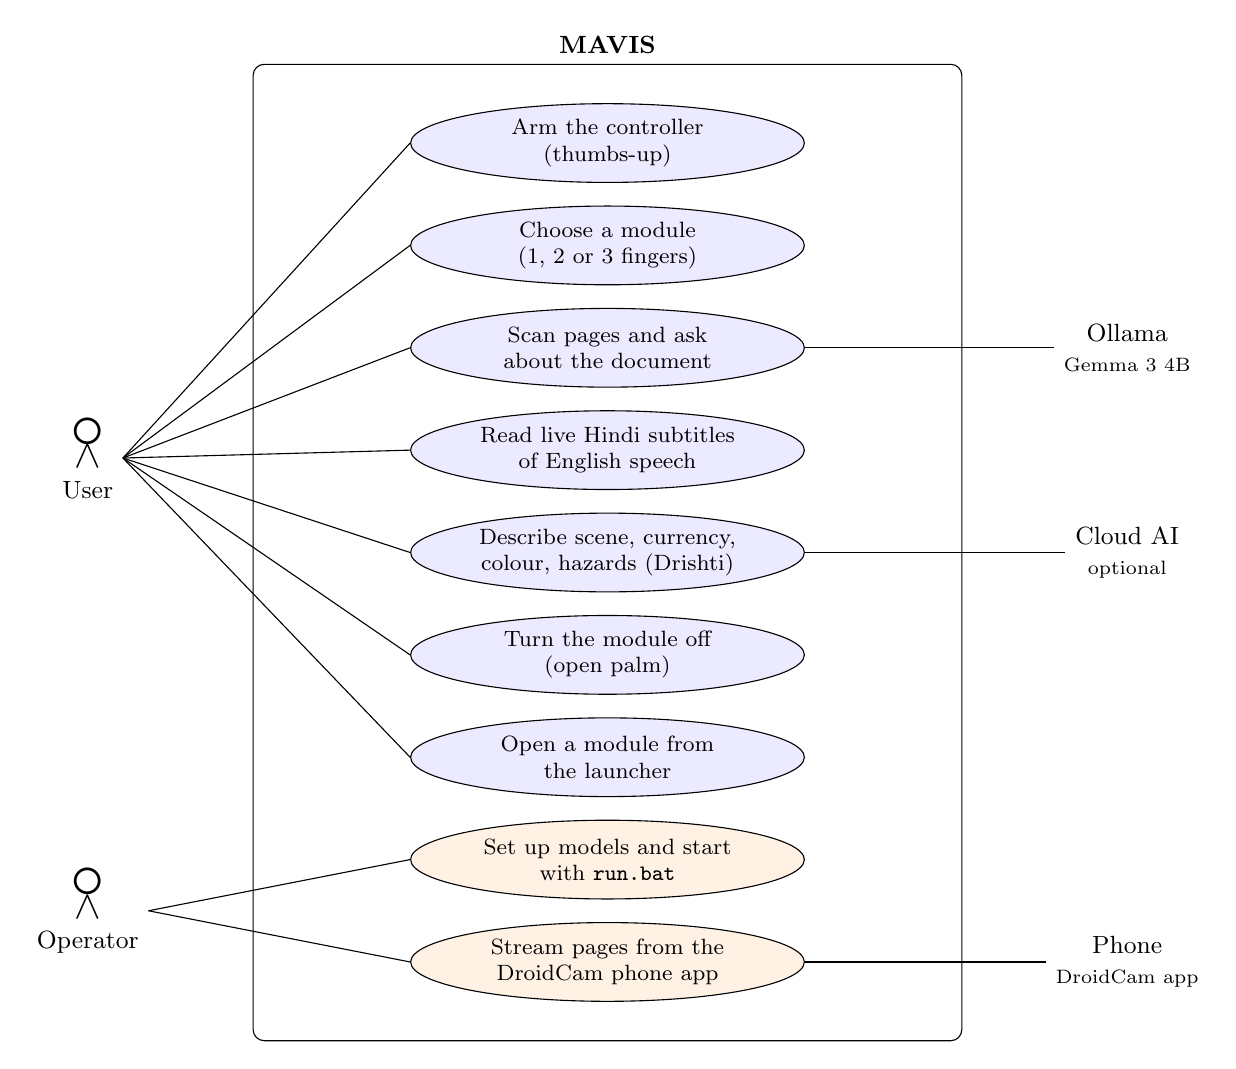
\begin{tikzpicture}[every node/.append style={execute at begin node={\hyphenpenalty=10000\exhyphenpenalty=10000}},font=\small,
  uc/.style={draw,ellipse,fill=mbsoft,minimum width=5.0cm,minimum height=1.0cm,align=center,inner sep=1pt,font=\footnotesize},
  actor/.style={align=center}]
\node[draw,rounded corners=4pt,minimum width=9.0cm,minimum height=12.4cm,label={[font=\small\bfseries]above:MAVIS}] (sys) at (0,0.4) {};
\node[uc] (u1) at (0,5.6) {Arm the controller\\(thumbs-up)};
\node[uc] (u2) at (0,4.3) {Choose a module\\(1, 2 or 3 fingers)};
\node[uc] (u3) at (0,3.0) {Scan pages and ask\\about the document};
\node[uc] (u4) at (0,1.7) {Read live Hindi subtitles\\of English speech};
\node[uc] (u5) at (0,0.4) {Describe scene, currency,\\colour, hazards (Drishti)};
\node[uc] (u6) at (0,-0.9) {Turn the module off\\(open palm)};
\node[uc] (u7) at (0,-2.2) {Open a module from\\the launcher};
\node[uc,fill=orange!10] (u8) at (0,-3.5) {Set up models and start\\with \texttt{run.bat}};
\node[uc,fill=orange!10] (u9) at (0,-4.8) {Stream pages from the\\DroidCam phone app};
\node[actor] (user) at (-6.6,1.6) {\Huge$\circ$\\[-4pt]\Large$\land$\\User};
\node[actor] (op) at (-6.6,-4.15) {\Huge$\circ$\\[-4pt]\Large$\land$\\Operator};
\node[actor] (oll) at (6.6,3.0) {Ollama\\{\scriptsize Gemma 3 4B}};
\node[actor] (cl) at (6.6,0.4) {Cloud AI\\{\scriptsize optional}};
\node[actor] (ph) at (6.6,-4.8) {Phone\\{\scriptsize DroidCam app}};
\foreach \u in {u1,u2,u3,u4,u5,u6,u7} \draw (user.east) -- (\u.west);
\draw (op.east) -- (u8.west); \draw (op.east) -- (u9.west);
\draw (u3.east) -- (oll.west); \draw (u5.east) -- (cl.west); \draw (u9.east) -- (ph.west);
\end{tikzpicture}
\caption{Use-case diagram}
\label{fig:usecase}
\end{figure}

\subsection{Data Flow Diagrams}
At level~0 MAVIS is one process on the laptop. It takes camera frames, microphone audio and questions from the user's browser and returns the active module and its results; it exchanges prompts with the local Ollama runtime and, only when configured, with cloud services. Level~1 (Figure~\ref{fig:dfd1}) splits it into its processes and stores.



\begin{figure}[H]
\centering
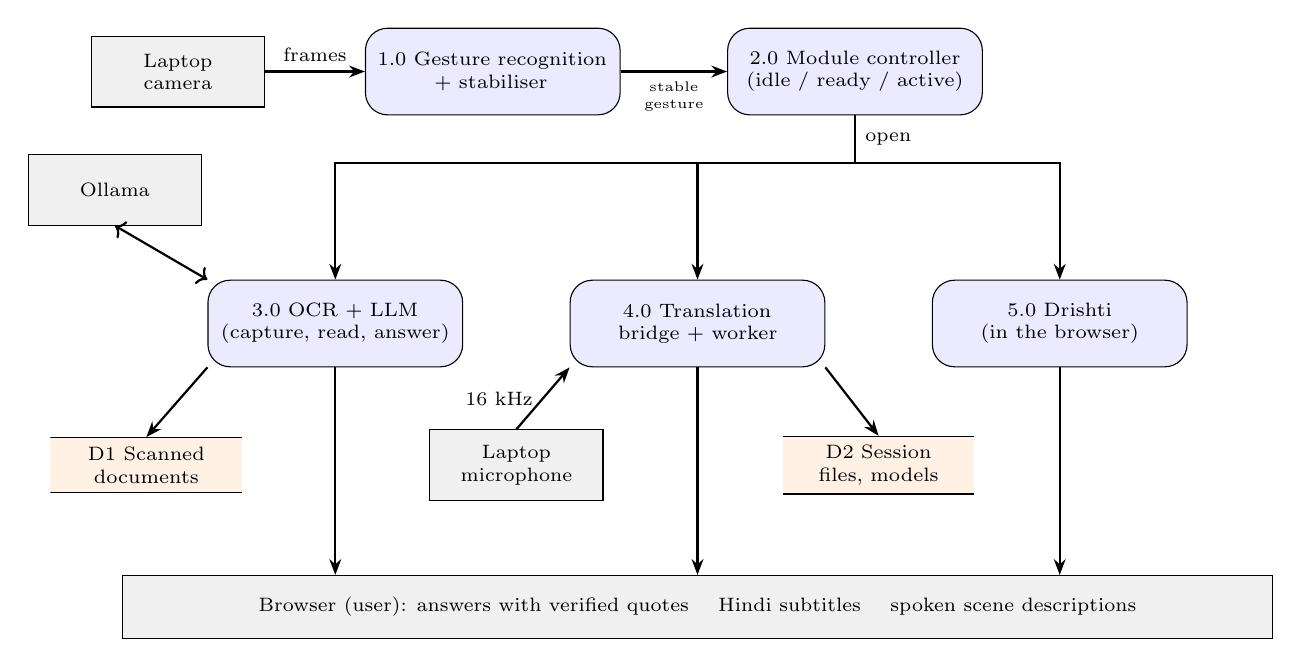
\begin{tikzpicture}[every node/.append style={execute at begin node={\hyphenpenalty=10000\exhyphenpenalty=10000}},font=\scriptsize,
  ent/.style={draw,fill=gray!12,minimum width=2.2cm,minimum height=0.9cm,align=center},
  proc/.style={draw,rounded corners=8pt,fill=mbsoft,text width=3.0cm,minimum height=1.1cm,align=center},
  store/.style={draw=none,fill=orange!10,text width=2.7cm,minimum height=0.7cm,align=center,path picture={\draw (path picture bounding box.north west)--(path picture bounding box.north east);\draw (path picture bounding box.south west)--(path picture bounding box.south east);}},
  arr/.style={-{Stealth[length=2mm]},thick}]
\node[ent] (cam) at (-6.6,3.2) {Laptop\\camera};
\node[proc] (p1) at (-2.6,3.2) {1.0 Gesture recognition\\+ stabiliser};
\node[proc] (p2) at (2.0,3.2) {2.0 Module controller\\(idle / ready / active)};
\node[proc] (p3) at (-4.6,0) {3.0 OCR + LLM\\(capture, read, answer)};
\node[proc] (p4) at (0,0) {4.0 Translation\\bridge + worker};
\node[proc] (p5) at (4.6,0) {5.0 Drishti\\(in the browser)};
\node[ent] (oll) at (-7.4,1.7) {Ollama};
\node[store,text width=2.2cm] (d1) at (-7.0,-1.8) {D1 Scanned documents};
\node[ent] (mic) at (-2.3,-1.8) {Laptop\\microphone};
\node[store,text width=2.2cm] (d2) at (2.3,-1.8) {D2 Session files, models};
\node[draw,fill=gray!12,minimum width=14.6cm,minimum height=0.8cm,align=center] (ui) at (0,-3.6) {Browser (user): answers with verified quotes \quad Hindi subtitles \quad spoken scene descriptions};
\draw[arr] (cam) -- node[above]{frames} (p1);
\draw[arr] (p1) -- node[below,font=\tiny,align=center]{stable\\gesture} (p2);
\draw[arr] (p2.south) -- node[right]{open} ++(0,-0.6) -| (p3.north);
\draw[arr] (p2.south) -- ++(0,-0.6) -| (p4.north);
\draw[arr] (p2.south) -- ++(0,-0.6) -| (p5.north);
\draw[arr,<->] (oll.south) -- (p3.north west);
\draw[arr] (p3.south west) -- (d1.north);
\draw[arr] (mic.north) -- node[left]{16 kHz} (p4.south west);
\draw[arr] (p4.south east) -- (d2.north);
\draw[arr] (p3.south) -- (p3.south |- ui.north);
\draw[arr] (p4.south) -- (p4.south |- ui.north);
\draw[arr] (p5.south) -- (p5.south |- ui.north);
\end{tikzpicture}
\caption{Data flow diagram, level 1 (camera frames also enter 3.0 and 5.0 in the browser)}
\label{fig:dfd1}
\end{figure}

\subsection{State Diagram: Module Controller}
The controller (Figure~\ref{fig:fsm}) has three states. It consumes only \emph{stabilised} gestures---one event per deliberate showing of a hand---so a hand passing through a pose does not change the state.

\begin{figure}[H]
\centering
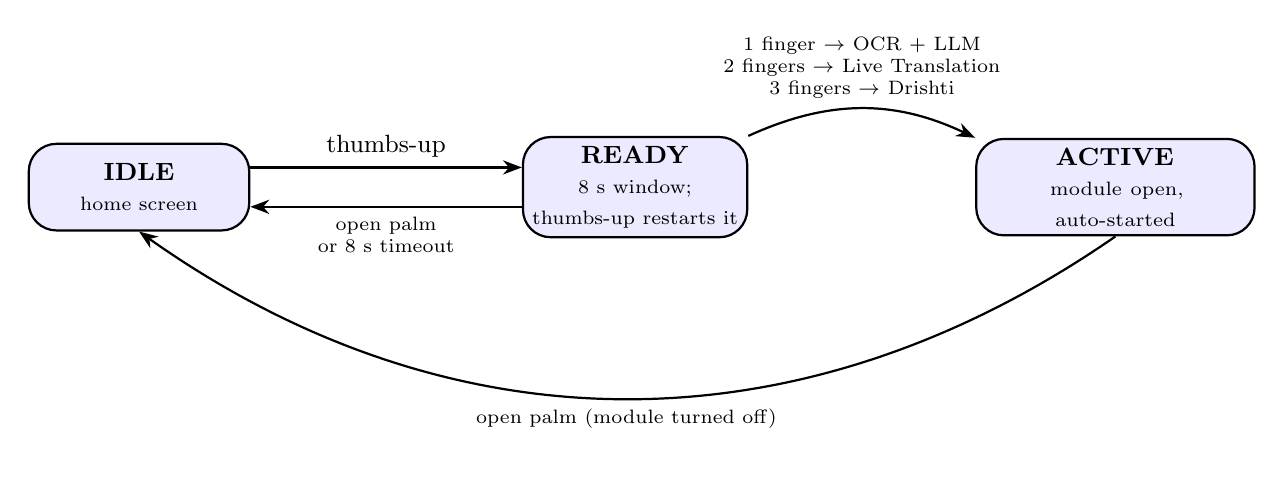
\begin{tikzpicture}[every node/.append style={execute at begin node={\hyphenpenalty=10000\exhyphenpenalty=10000}},font=\small,
  st/.style={draw,rounded corners=10pt,fill=mbsoft,minimum width=2.8cm,minimum height=1.1cm,align=center,thick},
  arr/.style={-{Stealth[length=2.4mm]},thick}]
\node[st] (idle) at (0,0) {\textbf{IDLE}\\{\scriptsize home screen}};
\node[st] (ready) at (6.3,0) {\textbf{READY}\\{\scriptsize 8 s window;}\\{\scriptsize thumbs-up restarts it}};
\node[st,text width=3.3cm] (act) at (12.4,0) {\textbf{ACTIVE}\\{\scriptsize module open,}\\{\scriptsize auto-started}};
\draw[arr] ([yshift=2.5mm]idle.east) -- node[above]{thumbs-up} ([yshift=2.5mm]ready.west);
\draw[arr] (ready.north east) to[bend left=25] node[above,align=center,font=\scriptsize]{1 finger $\to$ OCR + LLM\\2 fingers $\to$ Live Translation\\3 fingers $\to$ Drishti} (act.north west);
\draw[arr] ([yshift=-2.5mm]ready.west) -- node[below,font=\scriptsize,align=center]{open palm\\or 8 s timeout} ([yshift=-2.5mm]idle.east);
\draw[arr] (act.south) to[bend left=35] node[below,font=\scriptsize]{open palm (module turned off)} (idle.south);
\end{tikzpicture}
\caption{State diagram of the module controller}
\label{fig:fsm}
\end{figure}

\subsection{Sequence Diagram: Choosing a Module by Gesture}
Figure~\ref{fig:seq} follows one choice from the camera to a running module. The browser sends a JPEG frame about every 66\,ms; only one frame is in flight at a time, so frames never queue behind a slow one.

\begin{figure}[H]
\centering
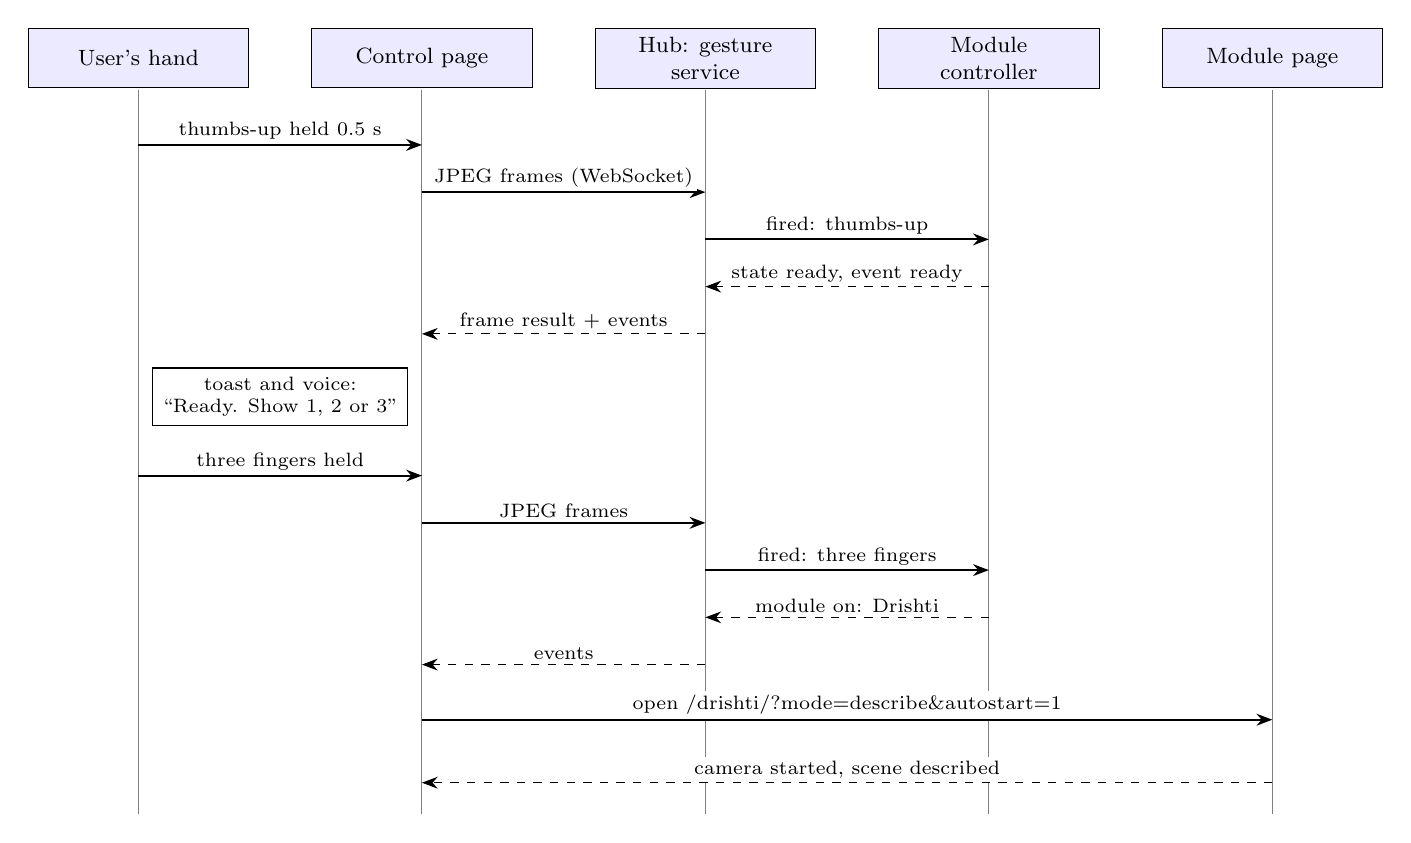
\begin{tikzpicture}[every node/.append style={execute at begin node={\hyphenpenalty=10000\exhyphenpenalty=10000}},font=\scriptsize,
  hd/.style={draw,fill=mbsoft,minimum width=2.8cm,minimum height=0.75cm,align=center,font=\footnotesize},
  msg/.style={-{Stealth[length=2mm]},thick},
  ret/.style={-{Stealth[length=2mm]},dashed},
  lb/.style={above,fill=white,inner sep=1.5pt}]
\foreach \x/\n/\t in {0/u/User's hand,3.6/b/Control page,7.2/h/Hub: gesture\\service,10.8/c/Module\\controller,14.4/m/Module page}{
  \node[hd] (\n) at (\x,0) {\t};
  \draw[gray] (\x,-0.4) -- (\x,-9.6);
}
\draw[msg] (0,-1.1) -- node[lb]{thumbs-up held 0.5 s} (3.6,-1.1);
\draw[msg] (3.6,-1.7) -- node[lb]{JPEG frames (WebSocket)} (7.2,-1.7);
\draw[msg] (7.2,-2.3) -- node[lb]{fired: thumbs-up} (10.8,-2.3);
\draw[ret] (10.8,-2.9) -- node[lb]{state ready, event ready} (7.2,-2.9);
\draw[ret] (7.2,-3.5) -- node[lb]{frame result + events} (3.6,-3.5);
\node[draw,fill=white,align=center,font=\scriptsize] at (1.8,-4.3) {toast and voice:\\``Ready. Show 1, 2 or 3''};
\draw[msg] (0,-5.3) -- node[lb]{three fingers held} (3.6,-5.3);
\draw[msg] (3.6,-5.9) -- node[lb]{JPEG frames} (7.2,-5.9);
\draw[msg] (7.2,-6.5) -- node[lb]{fired: three fingers} (10.8,-6.5);
\draw[ret] (10.8,-7.1) -- node[lb]{module on: Drishti} (7.2,-7.1);
\draw[ret] (7.2,-7.7) -- node[lb]{events} (3.6,-7.7);
\draw[msg] (3.6,-8.4) -- node[lb]{open /drishti/?mode=describe\&autostart=1} (14.4,-8.4);
\draw[ret] (14.4,-9.2) -- node[lb]{camera started, scene described} (3.6,-9.2);
\end{tikzpicture}
\caption{Sequence diagram: thumbs-up, then three fingers, opens Drishti}
\label{fig:seq}
\end{figure}

\subsection{Device Allocation}
Every module needs a camera, a microphone or both. Because a phone camera client may also be installed on the demonstration laptop, MAVIS fixes which device each module uses (Table~\ref{tab:devices}).

\begin{table}[H]
\centering
\caption{Camera and microphone used by each module}
\label{tab:devices}
\small
\begin{tabularx}{\textwidth}{@{}p{3.2cm}p{3.6cm}X@{}}
\toprule
\textbf{Module} & \textbf{Input} & \textbf{Source} \\
\midrule
Gesture control & Camera & Laptop camera (never DroidCam virtual camera) \\
OCR + LLM & Camera & User's choice on the module page: ``Use this device's camera'' (laptop camera) or the DroidCam phone app over Wi-Fi, entered as IP address and port; no default phone connection and no DroidCam Windows client needed \\
Live Translation & Microphone, camera & Laptop microphone for speech (system default unless it is a DroidCam device); laptop camera as the picture behind the subtitles \\
Drishti & Camera, microphone & Laptop camera and microphone (voice commands) \\
\bottomrule
\end{tabularx}
\end{table}
%=====================================================================
\section{Design and Methodology}
\subsection{Proposed System}
Figure~\ref{fig:arch} shows the block diagram. The gesture recognition module sits at the centre as the controller; the three assistance modules are equal peers that it opens. One Python process, the \emph{hub}, runs on the laptop and serves everything at \texttt{http://127.0.0.1:8000}: the launcher, the gesture control page, the OCR + LLM application (mounted under \texttt{/mavis/}), the translation subtitle page (\texttt{/translate/}) and Drishti (\texttt{/drishti/}). The translation package runs outside the hub, in its own Python environment, behind a small bridge process.

\begin{figure}[H]
\centering
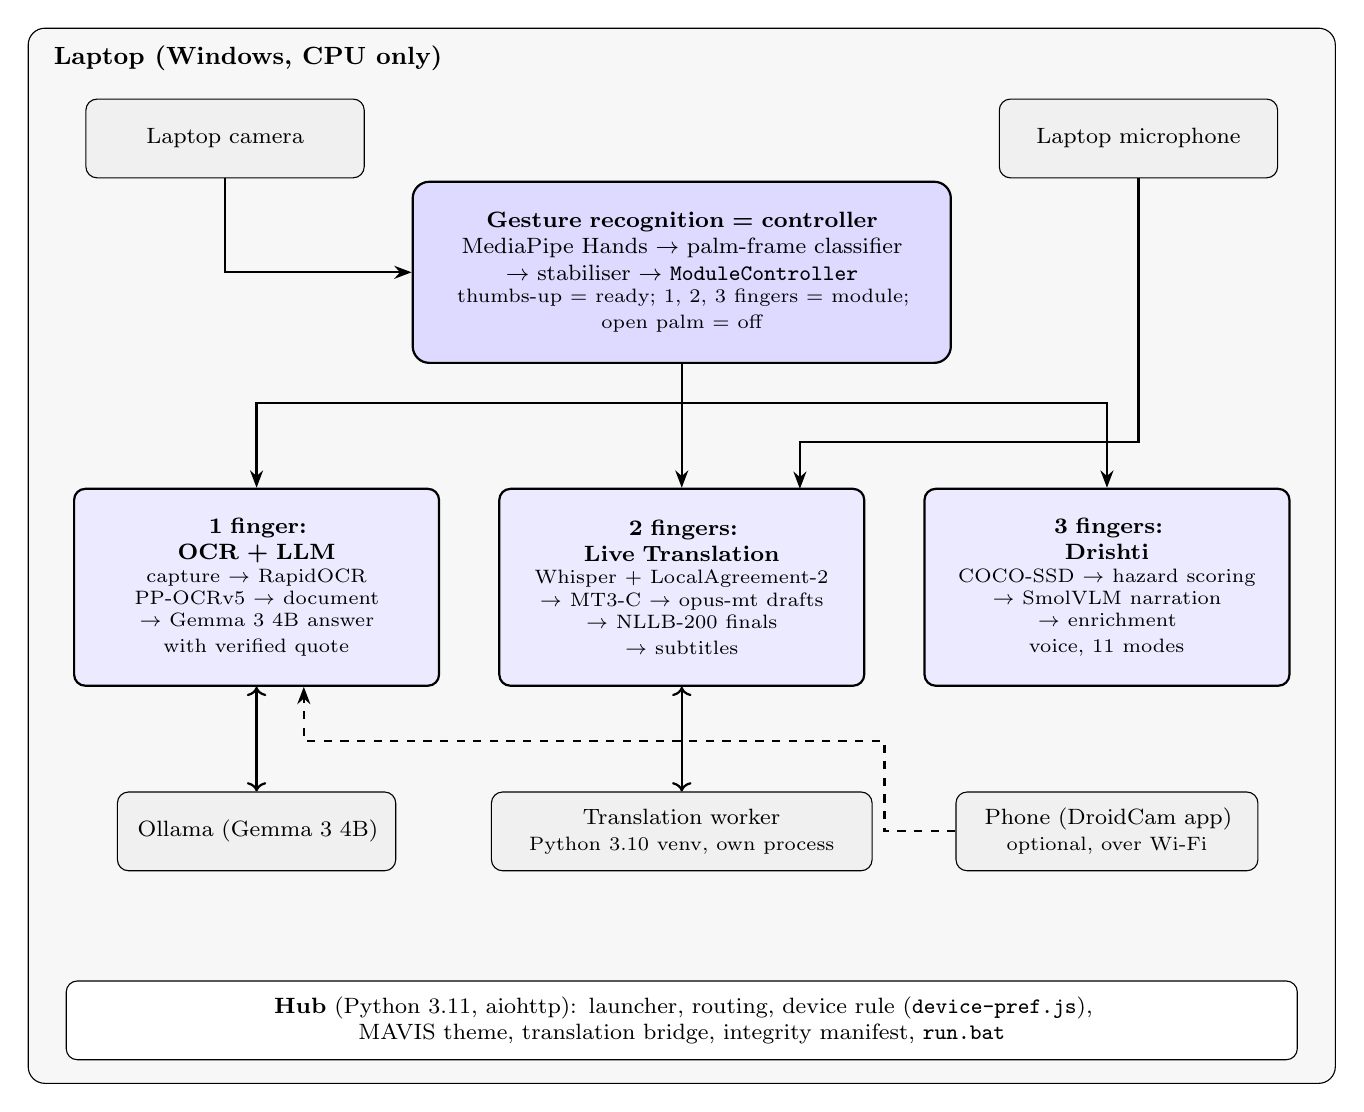
\begin{tikzpicture}[every node/.append style={execute at begin node={\hyphenpenalty=10000\exhyphenpenalty=10000}},font=\footnotesize,
  box/.style={draw,rounded corners=4pt,fill=white,text width=3.3cm,align=center,minimum height=1.0cm},
  mod/.style={draw,rounded corners=4pt,fill=mbsoft,text width=4.4cm,align=center,minimum height=2.5cm,thick,execute at begin node={\hyphenpenalty=10000}},
  arr/.style={-{Stealth[length=2.2mm]},thick}]
\node[draw,rounded corners=6pt,fill=gray!6,minimum width=16.6cm,minimum height=13.4cm] at (0,-1.0) {};
\node[font=\small\bfseries,anchor=north west] at (-8.1,5.6) {Laptop (Windows, CPU only)};
\node[box,fill=gray!12] (cam) at (-5.8,4.3) {Laptop camera};
\node[box,fill=gray!12] (mic) at (5.8,4.3) {Laptop microphone};
\node[draw,rounded corners=6pt,fill=mbrand!25,text width=6.6cm,align=center,minimum height=2.3cm,thick] (ctl) at (0,2.6)
 {\textbf{Gesture recognition = controller}\\MediaPipe Hands $\to$ palm-frame classifier $\to$ stabiliser $\to$ \texttt{ModuleController}\\{\scriptsize thumbs-up = ready; 1, 2, 3 fingers = module;\\open palm = off}};
\node[mod] (ocr) at (-5.4,-1.4) {\textbf{1 finger:}\\\textbf{OCR + LLM}\\{\scriptsize capture $\to$ RapidOCR\\PP-OCRv5 $\to$ document\\$\to$ Gemma 3 4B answer\\with verified quote}};
\node[mod] (tr) at (0,-1.4) {\textbf{2 fingers:}\\\textbf{Live Translation}\\{\scriptsize Whisper + LocalAgreement-2\\$\to$ MT3-C $\to$ opus-mt drafts\\$\to$ NLLB-200 finals\\$\to$ subtitles}};
\node[mod] (dr) at (5.4,-1.4) {\textbf{3 fingers:}\\\textbf{Drishti}\\{\scriptsize COCO-SSD $\to$ hazard scoring\\$\to$ SmolVLM narration\\$\to$ enrichment\\voice, 11 modes}};
\node[box,text width=15.4cm] (hub) at (0,-6.9) {\textbf{Hub} (Python 3.11, aiohttp): launcher, routing, device rule (\texttt{device-pref.js}), MAVIS theme, translation bridge, integrity manifest, \texttt{run.bat}};
\node[box,fill=gray!12] (oll) at (-5.4,-4.5) {Ollama (Gemma 3 4B)};
\node[box,fill=gray!12,text width=4.6cm] (venv) at (0,-4.5) {Translation worker\\{\scriptsize Python 3.10 venv, own process}};
\node[box,fill=gray!12,text width=3.6cm] (phone) at (5.4,-4.5) {Phone (DroidCam app)\\{\scriptsize optional, over Wi-Fi}};
\draw[arr] (cam) |- (ctl.west);
\draw[arr] (ctl.south) -- ++(0,-0.5) -| (ocr.north);
\draw[arr] (ctl.south) -- (tr.north);
\draw[arr] (ctl.south) -- ++(0,-0.5) -| (dr.north);
\draw[arr] (mic.south) -- (5.8,0.45) -- (1.5,0.45) -- (1.5,-0.15);
\draw[arr,<->] (ocr.south) -- (oll.north);
\draw[arr,<->] (tr.south) -- (venv.north);
\draw[arr,dashed] (phone.west) -- ++(-0.9,0) |- (-2.6,-3.35) -| ([xshift=6mm]ocr.south);
\end{tikzpicture}
\caption{Block diagram of MAVIS: the gesture controller opens one of three modules}
\label{fig:arch}
\end{figure}

Five design principles were followed. (1)~\emph{Integrate, do not modify}: each component is reached through its narrowest public boundary---the gesture pipeline's external-frame entry point, the OCR web application mounted as a sub-application, the translation package's documented host API, and Drishti's page served with an added script and stylesheet. (2)~\emph{The hand is the controller}: the controller decides which module runs; modules do not know about each other. (3)~\emph{One screen}: the chosen module opens inside the control page, with a small live view of the hand kept in the corner so that the off gesture is always visible. (4)~\emph{Predictable devices}: one rule decides which camera and microphone each module gets. (5)~\emph{One product}: one launcher, one colour scheme and one start command.

\subsection{Gesture Recognition and the Module Controller}
\subsubsection{Recognition Algorithm}
MediaPipe Hands \cite{zhang2020mediapipe,mediapipe_repo} returns 21 landmarks $\mathbf{p}_0,\dots,\mathbf{p}_{20}$ per hand. The recogniser expresses them in a palm frame with origin at the wrist $\mathbf{o}=\mathbf{p}_0$:
\begin{equation}
\mathbf{y}=\frac{\mathbf{p}_9-\mathbf{o}}{\lVert\mathbf{p}_9-\mathbf{o}\rVert},\quad
\mathbf{x}=\frac{\mathbf{t}-(\mathbf{t}\cdot\mathbf{y})\mathbf{y}}{\lVert\mathbf{t}-(\mathbf{t}\cdot\mathbf{y})\mathbf{y}\rVert},\ \mathbf{t}=\mathbf{p}_5-\mathbf{p}_{17},\quad
\mathbf{z}=c\,(\mathbf{x}\times\mathbf{y}),
\end{equation}
and $\mathbf{q}_i=A(\mathbf{p}_i-\mathbf{o})/s$ with $A=[\mathbf{x};\mathbf{y};\mathbf{z}]$, palm length $s=\lVert\mathbf{p}_9-\mathbf{o}\rVert$ and chirality $c=\pm1$. This makes the representation invariant to translation, scale and in-plane rotation and consistent for left and right hands. For each finger the summed joint bend $\Theta_f$ and the reach $r_f$ are mapped to $[0,1]$ by linear ramps and averaged into an extension score $e_f$; a finger with $e_f>0.6$ is \emph{extended} and one with $e_f<0.4$ \emph{folded}. Gestures are strict templates over the five finger states, with extra gates: spread fingers for an open palm, an upward thumb for thumbs-up, and rejection of edge-on palms.

\subsubsection{Temporal Stabilisation}
A gesture \emph{fires} only when it has been recognised in at least 5 consecutive frames with confidence $\geq 0.55$ and held for 0.5\,s; it fires once per showing, and a 0.8\,s cool-down follows. The controller consumes only these fired events, so it never reacts to a hand that merely passes through a pose.

\subsubsection{Module Controller}
\texttt{ModuleController} implements the state machine of Figure~\ref{fig:fsm} in about 80 lines of new code that sit beside, not inside, the recogniser. Table~\ref{tab:gmap} lists the mapping. Each frame's result is extended with the controller's events (\texttt{ready}, \texttt{module\_on}, \texttt{module\_off}, \texttt{ready\_timeout}, \texttt{ready\_cancelled}) and its state (including the seconds left in the ready window). The control page reacts to the events: it speaks and shows the change, opens the module's URL in a full-screen frame on the same page, and closes it on \texttt{module\_off}.

\begin{table}[H]
\centering
\caption{Gesture map of the controller}
\label{tab:gmap}
\small
\begin{tabularx}{\textwidth}{@{}p{3.2cm}p{2.4cm}X@{}}
\toprule
\textbf{Gesture} & \textbf{Valid in} & \textbf{Effect} \\
\midrule
Thumbs-up & Idle, Ready & Enter (or extend) the 8\,s ready window \\
One finger & Ready & Open OCR + LLM (\texttt{/mavis/}) \\
Two fingers & Ready & Open Live Translation (\texttt{/translate/?autostart=1}): listening starts automatically \\
Three fingers & Ready & Open Drishti (\texttt{/drishti/?mode=describe\&autostart=1}): camera starts and the first scene is described \\
Open palm & Ready, Active & Cancel the ready window, or turn the open module off and return home \\
\bottomrule
\end{tabularx}
\end{table}

\subsubsection{Camera and Output on the Same Screen}
The control page opens the laptop camera in the browser with \texttt{getUserMedia} \cite{w3cmediacapture} and sends JPEG frames ($640\times480$, quality 0.7) about every 66\,ms over the WebSocket \cite{rfc6455} \texttt{/hub/gesture/ws}. The hub gives each browser tab its own unchanged gesture pipeline on a single-thread executor (MediaPipe graphs are not thread-safe) and returns one JSON message per frame: the 21 landmarks, the gesture and confidence, the hold progress, and the controller state and events. The page draws the hand skeleton and a hold ring in the corner view. This replaced the recogniser's original OpenCV window on the desktop, so all gesture feedback now appears where the user is looking.

\subsection{Module 1 --- OCR + LLM}
\subsubsection{Pipeline}
Figure~\ref{fig:ocrpipe} shows the pipeline. (1)~\emph{Capture}: the ``smart'' selector captures a page a few seconds after the view changes and skips repeats; the sharpest frame of a short window is chosen by the variance of the Laplacian, and motion is detected with optical flow. The original manual four-point selection step was removed by its author after the benchmark below. (2)~\emph{OCR}: RapidOCR with PP-OCRv5 mobile \cite{du2020ppocr,rapidocr} on ONNX Runtime, whose differentiable-binarisation detector, direction classifier and CTC recogniser follow CRAFT \cite{baek2019} and CRNN \cite{shi2017}; a cloud vision reader can be used when a key is configured. (3)~\emph{Document}: pages are finalised into a multi-page document. (4)~\emph{Grounded answer}: following retrieval-augmented generation \cite{lewis2020}, Gemma~3 4B \cite{gemma3} in Ollama returns JSON with an answer and evidence items (page, exact quote). Because grounding alone does not prevent hallucination \cite{ji2023}, every quote is searched for in that page's OCR text, exactly and then approximately, and the answer is marked \emph{verified} only if its evidence is found.

\begin{figure}[H]
\centering
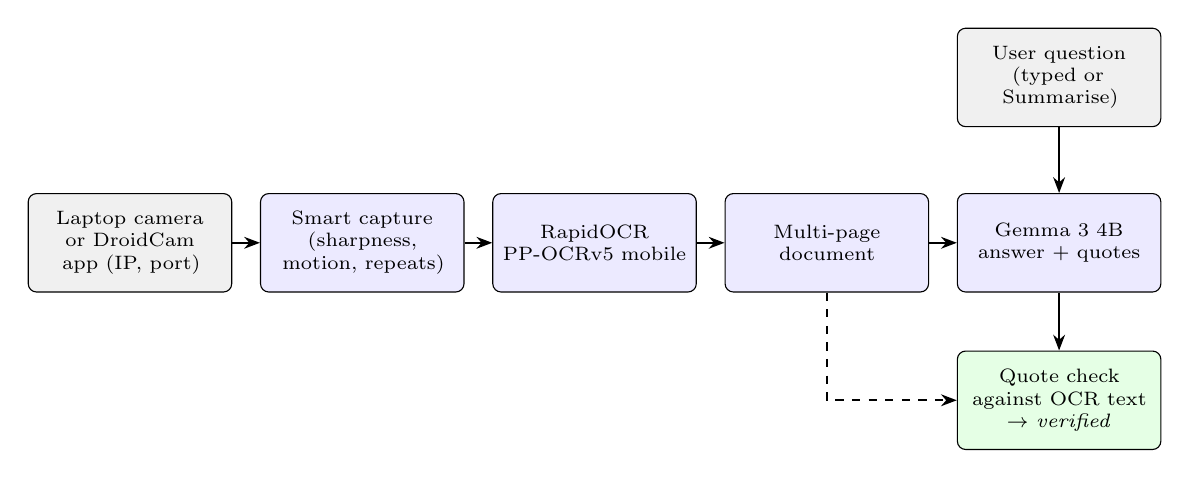
\begin{tikzpicture}[every node/.append style={execute at begin node={\hyphenpenalty=10000\exhyphenpenalty=10000}},font=\scriptsize,
  b/.style={draw,rounded corners=3pt,fill=mbsoft,text width=2.35cm,align=center,minimum height=1.25cm},
  arr/.style={-{Stealth[length=2mm]},thick}]
\node[b,fill=gray!12] (c) at (0,0) {Laptop camera\\or DroidCam app (IP, port)};
\node[b] (s) at (2.95,0) {Smart capture\\(sharpness, motion, repeats)};
\node[b] (o) at (5.9,0) {RapidOCR\\PP-OCRv5 mobile};
\node[b] (d) at (8.85,0) {Multi-page\\document};
\node[b] (q) at (11.8,0) {Gemma 3 4B\\answer + quotes};
\node[b,fill=green!10] (v) at (11.8,-2.0) {Quote check\\against OCR text\\$\to$ \emph{verified}};
\node[b,fill=gray!12] (u) at (11.8,2.1) {User question\\(typed or Summarise)};
\foreach \a/\bb in {c/s,s/o,o/d,d/q} \draw[arr] (\a) -- (\bb);
\draw[arr] (q) -- (v); \draw[arr] (u) -- (q);
\draw[arr,dashed] (d.south) |- (v.west);
\end{tikzpicture}
\caption{OCR + LLM pipeline}
\label{fig:ocrpipe}
\end{figure}

\subsubsection{Two Camera Paths}
The module's own scanning reads frames from \texttt{http://<ip>:<port>/video}, the MJPEG stream of the DroidCam phone app. The page therefore offers the user two choices, with no default: (a)~enter the phone's IP address and port to stream from the DroidCam app over Wi-Fi (no DroidCam Windows client is needed), or (b)~``Use this device's camera''. For (b) the hub \emph{acts as} a DroidCam: an added script sends the laptop camera's frames ($1920\times1080$, 15\,fps, JPEG 0.85) over a WebSocket, a loopback listener on port 8766 serves them as \texttt{multipart/x-mixed-replace} in DroidCam's format, and the hub starts the module's own scan with that address. Capture, OCR and question answering are therefore identical on both paths.

\subsection{Module 2 --- Live English-to-Hindi Translation}
\subsubsection{Streaming Pipeline}
The translation package (Figure~\ref{fig:trpipe}) is a cascade whose research core---M2 streaming recognition and the MT3-C scheduler---is frozen and protected by SHA-256 checks. Audio arrives in 100\,ms frames at 16\,kHz; Silero VAD \cite{silero} marks speech; a persistent streaming buffer builds a window after at least 2\,s of new audio; faster-whisper tiny (CPU, int8) \cite{radford2023} decodes it; and a prefix-agreement tracker implementing LocalAgreement-2 \cite{machacek2023} commits the words that two consecutive decodes agree on (\texttt{en\_committed}). The MT3-C scheduler, an adaptive-deadline policy, decides when newly committed English is worth translating and schedules opus-mt-en-hi \cite{tiedemann2020} drafts (\texttt{hi\_draft}). A segment closes on a sentence end after a pause, on length, or after 2.5\,s of silence; NLLB-200 600M \cite{nllb2022} converted to CTranslate2 int8 then translates the whole segment once (\texttt{hi\_final}), and a final is never replaced.

\begin{figure}[H]
\centering
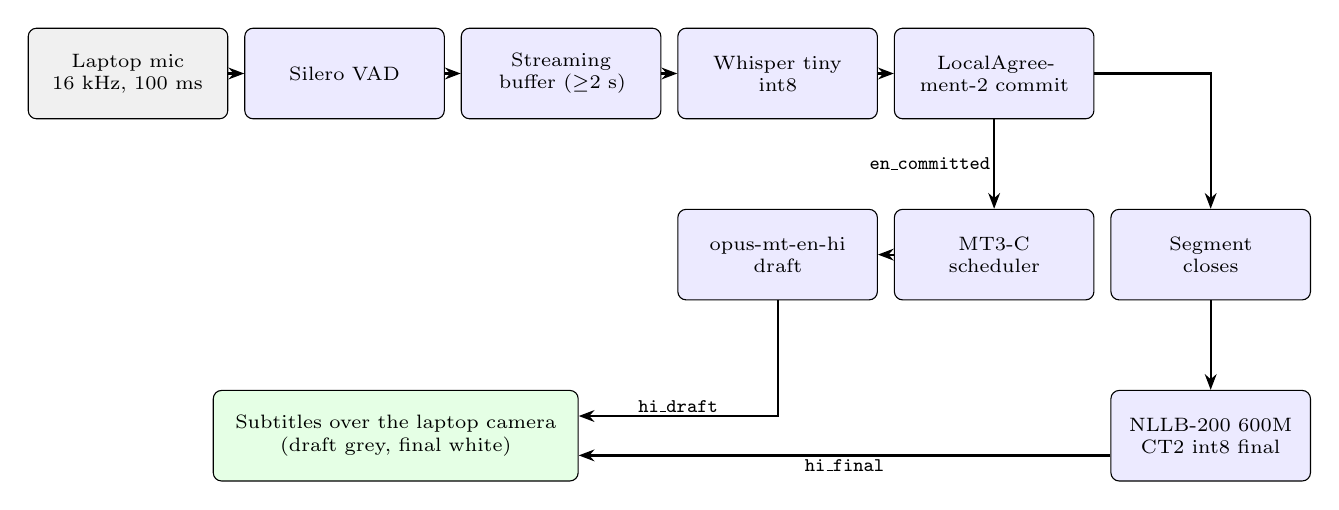
\begin{tikzpicture}[every node/.append style={execute at begin node={\hyphenpenalty=10000\exhyphenpenalty=10000}},font=\scriptsize,
  b/.style={draw,rounded corners=3pt,fill=mbsoft,text width=2.3cm,align=center,minimum height=1.15cm},
  arr/.style={-{Stealth[length=2mm]},thick}]
\node[b,fill=gray!12] (m) at (0,0) {Laptop mic\\16 kHz, 100 ms};
\node[b] (v) at (2.75,0) {Silero VAD};
\node[b] (sb) at (5.5,0) {Streaming\\buffer ($\geq$2 s)};
\node[b] (w) at (8.25,0) {Whisper tiny\\int8};
\node[b] (la) at (11.0,0) {LocalAgree-\\ment-2 commit};
\node[b] (s3) at (11.0,-2.3) {MT3-C\\scheduler};
\node[b] (op) at (8.25,-2.3) {opus-mt-en-hi\\draft};
\node[b] (sc) at (13.75,-2.3) {Segment\\closes};
\node[b] (nl) at (13.75,-4.6) {NLLB-200 600M\\CT2 int8 final};
\node[b,fill=green!10,text width=4.4cm] (sub) at (3.4,-4.6) {Subtitles over the laptop camera\\(draft grey, final white)};
\foreach \a/\bb in {m/v,v/sb,sb/w,w/la} \draw[arr] (\a) -- (\bb);
\draw[arr] (la) -- node[left,fill=white,inner sep=1pt]{\texttt{en\_committed}} (s3);
\draw[arr] (s3) -- (op);
\draw[arr] (la.east) -| (sc.north);
\draw[arr] (sc) -- (nl);
\draw[arr] (op.south) |- node[above,pos=0.75,fill=white,inner sep=1pt]{\texttt{hi\_draft}} ([yshift=2.5mm]sub.east);
\draw[arr] ([yshift=-2.5mm]nl.west) -- node[below,fill=white,inner sep=1pt]{\texttt{hi\_final}} ([yshift=-2.5mm]sub.east);
\end{tikzpicture}
\caption{Live translation pipeline (frozen core in the translation package)}
\label{fig:trpipe}
\end{figure}

\subsubsection{Integration Through the Host API}
The package exposes a host API, \texttt{create\_host\_session(SessionOptions(...))}, that starts one worker process per session and publishes events with schema \texttt{mavis.live\_translation.v1}, each with a session id and sequence number. Because the package needs its own pinned environment (Python~3.10, PyTorch CPU, CTranslate2, faster-whisper), the hub does not import it. Instead, the chain is subtitle page $\leftrightarrow$ hub (WebSocket) $\leftrightarrow$ bridge process (JSON lines on stdin/stdout) $\leftrightarrow$ worker process (host API):
\begin{itemize}[leftmargin=*]
\item \texttt{TranslationManager} in the hub checks that the package, its environment and its models are present, and starts \texttt{translation\_bridge.py} with the package's own Python interpreter, without a console window.
\item The bridge writes a host configuration with live translation enabled, chooses the microphone (the system default, unless that is a DroidCam device, in which case the first other input that accepts 16\,kHz), creates the session through the host API, and relays every event to the hub as one JSON line on standard output; it reads \texttt{start}/\texttt{stop} commands on standard input.
\item The hub keeps the session's event history and fans events out to browsers over \texttt{/hub/translation/ws}; when the last viewer disconnects, the session is stopped so the worker's memory is released.
\end{itemize}



\subsubsection{Subtitle Presentation}
The subtitle page fills the screen with the live laptop camera picture and shows only the current line, bottom centre, in large white text with a dark outline---as in a film. A Hindi draft is shown in a lighter tone and replaced by the final, which disappears after 7\,s. Following the package's event contract, events from other sessions and repeated sequence numbers are dropped and late drafts never replace a final. An \textbf{EN} button adds the English line above the Hindi, and a \textbf{Transcript} drawer keeps the whole conversation. When opened by gesture, the page starts the session automatically.

\subsection{Module 3 --- Drishti}
Drishti answers each request through a four-stage, local-first pipeline (Figure~\ref{fig:drpipe}). Stage~1 runs COCO-SSD \cite{liu2016ssd,sandler2018} (TensorFlow.js) in the browser with a 0.66 confidence floor. Stage~2 is deterministic: each box is given a clock position, a bucketed proximity (very close, close, medium, far), an in-path flag, and a hazard score
\begin{equation}
\text{risk} = w_{\text{class}} \times f_{\text{proximity}} \times f_{\text{path}} \times f_{\text{motion}},
\end{equation}
mapped to LOW, MEDIUM, HIGH or CRITICAL, together with a distance-confidence tag. Stage~3, SmolVLM-500M \cite{marafioti2025} through Transformers.js, writes the scene narration on the device. Stage~4 appends the measured positions and a local dominant-colour reading, so the spoken answer combines generated narration with explainable measurements. Cloud models (Groq, then Gemini or Cloudflare) are used only in Hybrid or Cloud mode and only for requests the local stack cannot answer.

\begin{figure}[H]
\centering
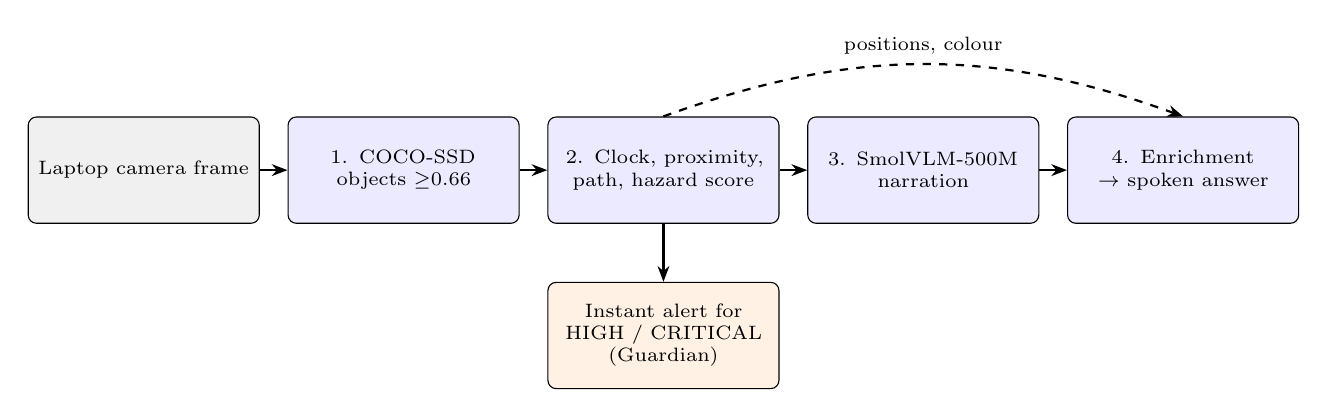
\begin{tikzpicture}[every node/.append style={execute at begin node={\hyphenpenalty=10000\exhyphenpenalty=10000}},font=\scriptsize,
  b/.style={draw,rounded corners=3pt,fill=mbsoft,text width=2.7cm,align=center,minimum height=1.35cm},
  arr/.style={-{Stealth[length=2mm]},thick}]
\node[b,fill=gray!12] (c) at (0,0) {Laptop camera frame};
\node[b] (s1) at (3.3,0) {1. COCO-SSD\\objects $\geq$0.66};
\node[b] (s2) at (6.6,0) {2. Clock, proximity, path, hazard score};
\node[b] (s3) at (9.9,0) {3. SmolVLM-500M narration};
\node[b] (s4) at (13.2,0) {4. Enrichment\\$\to$ spoken answer};
\node[b,fill=orange!10] (al) at (6.6,-2.1) {Instant alert for HIGH / CRITICAL (Guardian)};
\foreach \a/\bb in {c/s1,s1/s2,s2/s3,s3/s4} \draw[arr] (\a) -- (\bb);
\draw[arr] (s2) -- (al);
\draw[arr,dashed] (s2.north) to[bend left=20] node[above]{positions, colour} (s4.north);
\end{tikzpicture}
\caption{Drishti's four-stage local-first pipeline}
\label{fig:drpipe}
\end{figure}

\subsubsection{Features Kept in MAVIS}
Drishti originally had thirteen camera modes. Its \emph{Read Text} and \emph{Translate} modes duplicate the OCR + LLM and Live Translation modules, so MAVIS hides exactly those two buttons (\texttt{\#pill-text} and \texttt{\#pill-translate}) with an added script; voice commands that would switch to them are redirected. Table~\ref{tab:drfeat} lists what remains.

\begin{table}[H]
\centering
\caption{Drishti features kept in MAVIS}
\label{tab:drfeat}
\small
\begin{tabularx}{\textwidth}{@{}p{3.4cm}X@{}}
\toprule
\textbf{Feature} & \textbf{What it does} \\
\midrule
Describe & Scene narration from SmolVLM, enriched with real object positions and colours (default mode when opened by gesture) \\
Currency & Indian note denomination from local OCR of the printed value, cross-checked against the note's colour \\
Colour & Instant local $3\times3$ dominant-colour reading \\
Objects, Navigate & Detected objects with clock positions; path state CLEAR / OBSTACLE\_AHEAD / UNCERTAIN, never ``safe'' \\
Prices & Names the real detected items and declines to invent prices \\
People, Food & Semantic descriptions (cloud fallback when enabled) \\
Safety, Crossing & Hazard observations; Crossing reports CLEAR\_VIEW or UNCLEAR\_VIEW with a fixed disclaimer, never GO \\
Gesture & Drishti's own sign/gesture description mode \\
Guardian, Sound alerts & Continuous hazard alerts; YAMNet sound-hazard alerts \\
Smart Live, Snap, Ask Drishti & Continuous or single-shot analysis; questions about the current view \\
Voice and SOS & Voice commands and replies in English and eight Indian languages; SOS button \\
\bottomrule
\end{tabularx}
\end{table}

\subsubsection{Auto-Start}
When opened as \texttt{/drishti/?mode=describe\&autostart=1}, the added script selects the mode through Drishti's own \texttt{setMode} function, starts the camera with Drishti's own \texttt{startCam}, and triggers the first \texttt{snap}, so the user hears a description without touching anything.

\subsection{Integration Methodology}
\subsubsection{Zero Modification and Integrity}
All adaptation happens at the boundary: new routes in the hub, scripts and stylesheets injected into the served pages, the bridge process for translation, and environment variables that the components already document. A manifest, \texttt{ORIGINALS.sha256}, records the digest of all 314 original files (234 from the gesture, OCR and Drishti projects and 80 from the translation package); \texttt{python -m hub.verify\_originals} re-checks them. Git attributes mark the translation package as binary so that line endings---part of its frozen hashes---are never converted.

\subsubsection{Device Rule}
\texttt{device-pref.js} is loaded first on every page. It wraps \texttt{getUserMedia}: when a page asks for a camera or microphone without naming one and a DroidCam virtual device is present, it requests the first non-DroidCam device instead. Because browsers hide device names until the first permission, the choice is repeated once names are visible. A page that names a device (the OCR module's camera button) gets exactly that device, and if the chosen device fails the browser default is used.

\subsubsection{One Colour Scheme}
\texttt{mavis-theme.css} defines one dark palette (background \#0D1117, surfaces \#151B26--\#243045, text \#E8EDF5, brand violet \#7C6CFF, and status colours) and maps every component's own CSS variables onto it. The rule uses \texttt{html:root}, which is more specific than each component's \texttt{:root}, so it wins in light and dark mode alike without editing their stylesheets; a few colours that Drishti hard-codes are overridden by scoped selectors.

\subsubsection{Packaging}
\texttt{setup.bat} creates the hub environment from a single lock file (one OpenCV build, \texttt{opencv-contrib-python}, shared by the OCR and gesture code); \texttt{setup\_translation.bat} runs the package's own setup and model download, with a wrapper that disables Hugging Face symbolic links, which fail on Windows without developer mode. \texttt{run.bat} starts Ollama if it is installed and not running, loads optional keys, starts the hub and opens the launcher---the only step needed for the demonstration.

\subsection{Models and Datasets Used}
\begin{table}[H]
\centering
\caption{Pre-trained models and datasets used}
\label{tab:data}
\small
\begin{tabularx}{\textwidth}{@{}p{3.9cm}p{2.5cm}X@{}}
\toprule
\textbf{Model / dataset} & \textbf{Module} & \textbf{Use} \\
\midrule
MediaPipe Hands \cite{zhang2020mediapipe} & Controller & 21-landmark hand tracking (pre-trained, not retrained) \\
HaGRID \cite{kapitanov2024} & Controller (tests) & Real hand photographs turned into camera video for end-to-end tests \\
PP-OCRv5 mobile \cite{du2020ppocr} & OCR + LLM & Text detection, orientation and recognition through RapidOCR \\
Gemma~3 4B \cite{gemma3} & OCR + LLM & Local grounded question answering (Ollama) \\
Printed test pages & OCR + LLM (tests) & Invoice, sales table and meeting minutes photographed on a desk \\
Silero VAD \cite{silero} & Translation & Speech / silence detection \\
Whisper tiny \cite{radford2023} & Translation & Streaming English recognition (faster-whisper, CPU int8) \\
opus-mt-en-hi \cite{tiedemann2020} & Translation & Fast Hindi drafts \\
NLLB-200 distilled 600M \cite{nllb2022} & Translation & Final Hindi translation per segment (CTranslate2 int8) \\
300-file speech corpus & Translation (eval.) & 1105.8\,s of English speech for the M1/M2 comparison (black book) \\
COCO-SSD \cite{liu2016ssd,sandler2018} & Drishti & On-device object detection \\
SmolVLM-500M \cite{marafioti2025} & Drishti & On-device scene narration \\
Tesseract.js \cite{smith2007}, YAMNet, Depth-Anything & Drishti & Currency digits, sound alerts, on-demand distance \\
\bottomrule
\end{tabularx}
\end{table}

\subsection{Testing Methodology}
Testing has five layers. (1)~\emph{Regression}: each component's own test suite, unchanged, in its environment. (2)~\emph{Integrity}: the manifest check. (3)~\emph{Integration tests} (21) for the new code: the controller's transitions and timeouts, the gesture service with recorded real landmarks, the translation bridge against a stand-in package with the same host API, the relay, routes and access rules. (4)~\emph{Browser end-to-end tests} in Chromium driven by Playwright, with real photographs (HaGRID hand photos \cite{kapitanov2024} and printed pages) converted to video and played as the browser's camera. (5)~\emph{Live tests} on the demonstration laptop with its real camera, microphone and the DroidCam app. Measured results of each component's own research evaluations are reported from its black book and labelled as such.
%=====================================================================
\section{Results and Discussion}
\subsection{Test Environment}
Integration and end-to-end tests ran on a 2-vCPU Linux machine without a GPU, in fresh environments built from the lock files, with headless Chromium (Playwright) whose camera was fed from video files made of real photographs. The complete system was then installed from the repository on the demonstration laptop (Windows, CPU only, Brave browser), where every module was tested live with the built-in camera and microphone and with the DroidCam phone app. Results of each component's own research evaluation were measured by its author and are reproduced from the team's black books; they are marked ``(black book)''.

\subsection{Code Preservation and Regression}
\texttt{python -m hub.verify\_originals} reported \textbf{314 original files intact, 0 changed, 0 missing}. Table~\ref{tab:regress} lists the test suites.

\begin{table}[H]
\centering
\caption{Regression and integration test results}
\label{tab:regress}
\small
\begin{tabularx}{\textwidth}{@{}p{4.8cm}p{3.6cm}X@{}}
\toprule
\textbf{Suite} & \textbf{Environment} & \textbf{Result} \\
\midrule
Gesture recognition (original) & Hub, Python 3.11 & 112 passed \\
OCR + LLM (original) & Hub, Python 3.11 & 149 passed, 5 skipped \\
Live translation package (original) & Package, Python 3.10 & 120 passed, 3 skipped (historical recordings not packaged) \\
Integrity manifest & --- & 314 / 314 files byte-identical \\
MAVIS integration tests (new) & Hub, Python 3.11 & 21 passed \\
\bottomrule
\end{tabularx}
\end{table}

\subsection{Gesture Controller}
\subsubsection{Recognition on Real Hand Photographs}
Real photographs from HaGRID \cite{kapitanov2024} were passed through the unchanged recogniser, as presented and mirrored (Table~\ref{tab:realhands}). All five controller gestures are recognised with confidence 0.79--1.00; the fist is rejected; a mirrored thumbs-up whose fingers are not curled is rejected rather than guessed. Four fingers is read as an open palm in one orientation, which in MAVIS only turns a module off---a safe failure.

\begin{table}[H]
\centering
\caption{Recogniser output on real hand photographs (confidence in brackets)}
\label{tab:realhands}
\small
\begin{tabular}{@{}lll@{}}
\toprule
\textbf{Photograph} & \textbf{As presented} & \textbf{Mirrored} \\
\midrule
One finger & \texttt{one\_finger} (0.79) & \texttt{one\_finger} (0.87) \\
Two fingers & \texttt{two\_fingers} (0.84) & \texttt{two\_fingers} (0.82) \\
Three fingers & \texttt{three\_fingers} (0.84) & \texttt{three\_fingers} (0.84) \\
Thumbs up & \texttt{thumbs\_up} (1.00) & UNKNOWN (fingers not curled) \\
Open palm & \texttt{open\_palm} (0.99) & \texttt{open\_palm} (0.98) \\
Fist (negative) & UNKNOWN (fist) & UNKNOWN (fist) \\
Four fingers (negative) & \texttt{open\_palm} (0.74) & UNKNOWN \\
\bottomrule
\end{tabular}
\end{table}

\subsubsection{End-to-End Control}
A video of real hands (thumbs-up, then three fingers, then open palm) was played as the camera of the gesture control page. Table~\ref{tab:ctle2e} shows what the page displayed; no page errors occurred. Each gesture took effect after its 0.5\,s hold, the module opened with its auto-start address, and the open palm closed it and returned to the home screen. The one- and two-finger paths, the 8\,s timeout and the cancel gesture are covered by the controller's integration tests.

\begin{table}[H]
\centering
\caption{End-to-end controller run in the browser (times from pressing Start camera)}
\label{tab:ctle2e}
\small
\begin{tabularx}{\textwidth}{@{}p{1.3cm}p{4.6cm}X@{}}
\toprule
\textbf{Time} & \textbf{Controller state shown} & \textbf{Page} \\
\midrule
0.3\,s & Idle --- thumbs-up to start & Home screen \\
2.1\,s & Ready (8\,s) --- show 1, 2 or 3 & Toast and voice ``Ready. Show one, two or three fingers'' \\
3.3--5.2\,s & Ready (7\,s \dots\ 5\,s) & Countdown on the home screen \\
5.8\,s & Drishti on --- open palm to turn off & \texttt{/drishti/?mode=describe\&autostart=1} opened; ``Starting Drishti'' \\
8.6\,s & Drishti on & Drishti camera running in Describe mode \\
10.7\,s & Idle & Module closed; ``Drishti turned off'' \\
\bottomrule
\end{tabularx}
\end{table}



\begin{figure}[H]
\centering
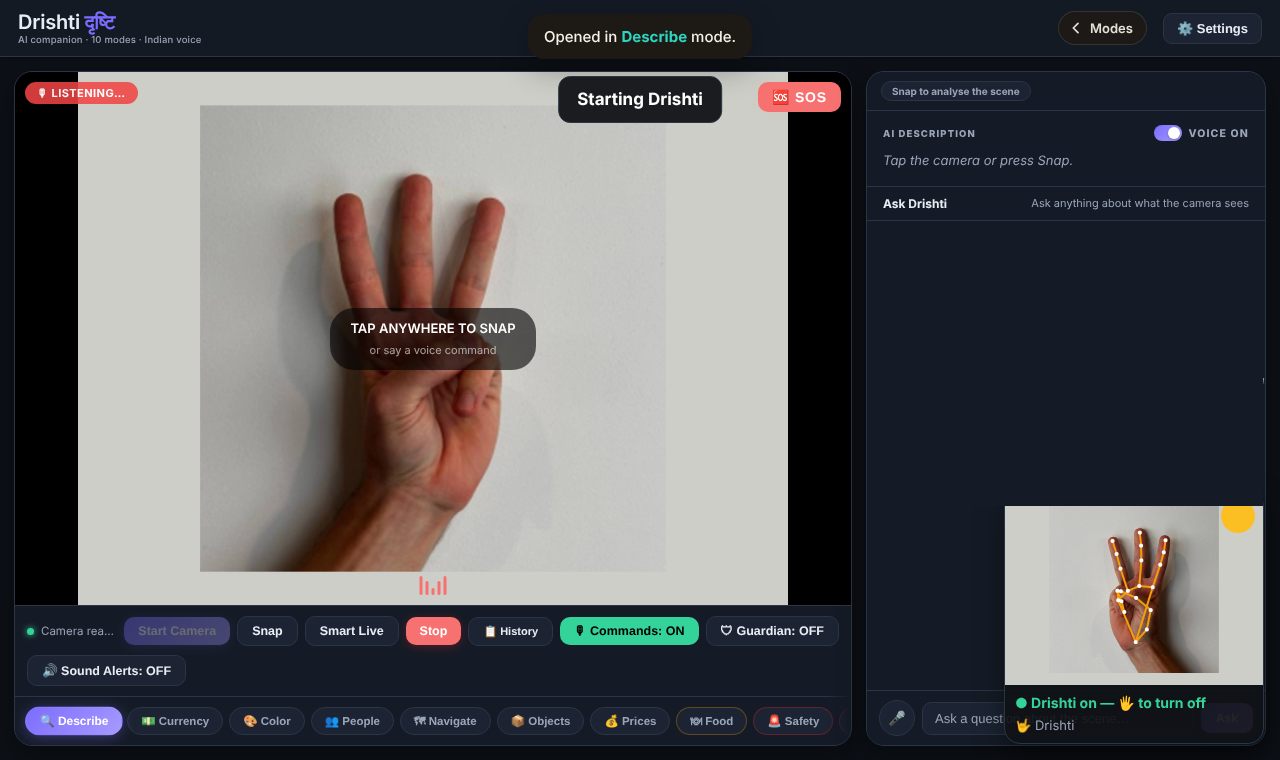
\includegraphics[width=0.6\textwidth]{f_control_drishti.png}
\caption{Three fingers opened Drishti, which started its camera in Describe mode; the live hand view (bottom right) shows the controller state}
\label{fig:ctldrishti}
\end{figure}

\subsubsection{Performance}
Over 140 frames of real hands the hub's time per frame (decode, track, classify, stabilise, controller, serialise) was mean 13.1\,ms, median 12.0\,ms, p95 18.4\,ms, against a 66\,ms interval between frames. A $640\times480$ frame at JPEG quality 0.7 is 12.7--14.9\,KB, about 0.2\,MB/s at 15 frames per second. Since only one frame is in flight, the delay seen by the user is the processing time plus one local round trip, plus the 0.5\,s hold that is deliberately required.

\subsection{OCR + LLM}
\subsubsection{Engine Selection Benchmark (black book)}
The OCR engine was chosen by a two-round benchmark of 12 candidates on frames of real documents, run one at a time on a CPU-only laptop. Round~2 (Table~\ref{tab:ocrbench}) used 30 deliberately harder frames: five documents, page turns, motion blur, a page rotated by 25--30$^\circ$, hand occlusion and one upside-down page.

\begin{table}[H]
\centering
\caption{OCR benchmark, Round 2, 30 frames (black book)}
\label{tab:ocrbench}
\small
\begin{tabular}{@{}lrrrrr@{}}
\toprule
\textbf{Model} & \textbf{Frames} & \textbf{Peak RSS (MB)} & \textbf{Avg (s)} & \textbf{p95 (s)} & \textbf{Catastrophic} \\
\midrule
RapidOCR PP-OCRv5 mobile & 30/30 & 295 & 4.59 & 5.76 & 0/30 \\
RapidOCR PP-OCRv5 (downscaled) & 30/30 & 286 & 4.74 & 6.13 & 0/30 \\
RapidOCR PP-OCRv4 mobile & 30/30 & 292 & 8.92 & 12.63 & 0/30 \\
docTR DB-Mobile + CRNN-small & 30/30 & 1746 & 1.22 & 1.49 & 6/30 \\
docTR FAST + CRNN-small & 30/30 & 1828 & 1.62 & 1.83 & 6/30 \\
docTR FAST + CRNN-large & 30/30 & 1914 & 3.81 & 5.10 & 6/30 \\
Granite-Docling-258M & 8/30 & --- & 51.07 & 77.44 & stopped \\
\bottomrule
\end{tabular}
\end{table}

docTR was faster but produced catastrophic hallucinated output on 20\% of frames in all three variants; RapidOCR PP-OCRv5 produced none, read the upside-down page as well as the upright one thanks to its orientation classifier, and recovered partial text under 70\% hand occlusion without fabricating values. Its cost grows with the amount of real text on the page (1.85\,s average in Round~1, 4.59\,s in Round~2), which is why it was selected despite being slower.

\subsubsection{Validation (black book)}
After the switch to automatic full-frame capture, the module's 27 unit and regression tests passed at every checkpoint; all 40 archived benchmark frames passed through the production path with 0 errors and 0 schema violations; and a live DroidCam session captured \textbf{23/23 pages with 0 OCR errors} and no fabricated text. Live OCR time over 21 pages was 3168\,ms average, 2780\,ms median and 5316\,ms p95; duplicate-frame filtering rejected 9 of 32 checked frames while the camera was still.

\subsubsection{In MAVIS}
Both camera paths reached the module's own scan: the laptop camera through the relay ($1920\times1080$ frames received intact), and the DroidCam app over Wi-Fi on the demonstration laptop. With printed test pages (an invoice, a sales table, meeting minutes), questions were answered by the local Gemma~3 4B model with page-cited quotes marked verified (Figures~\ref{fig:ocr} and~\ref{fig:answer}).

\begin{figure}[H]
\centering
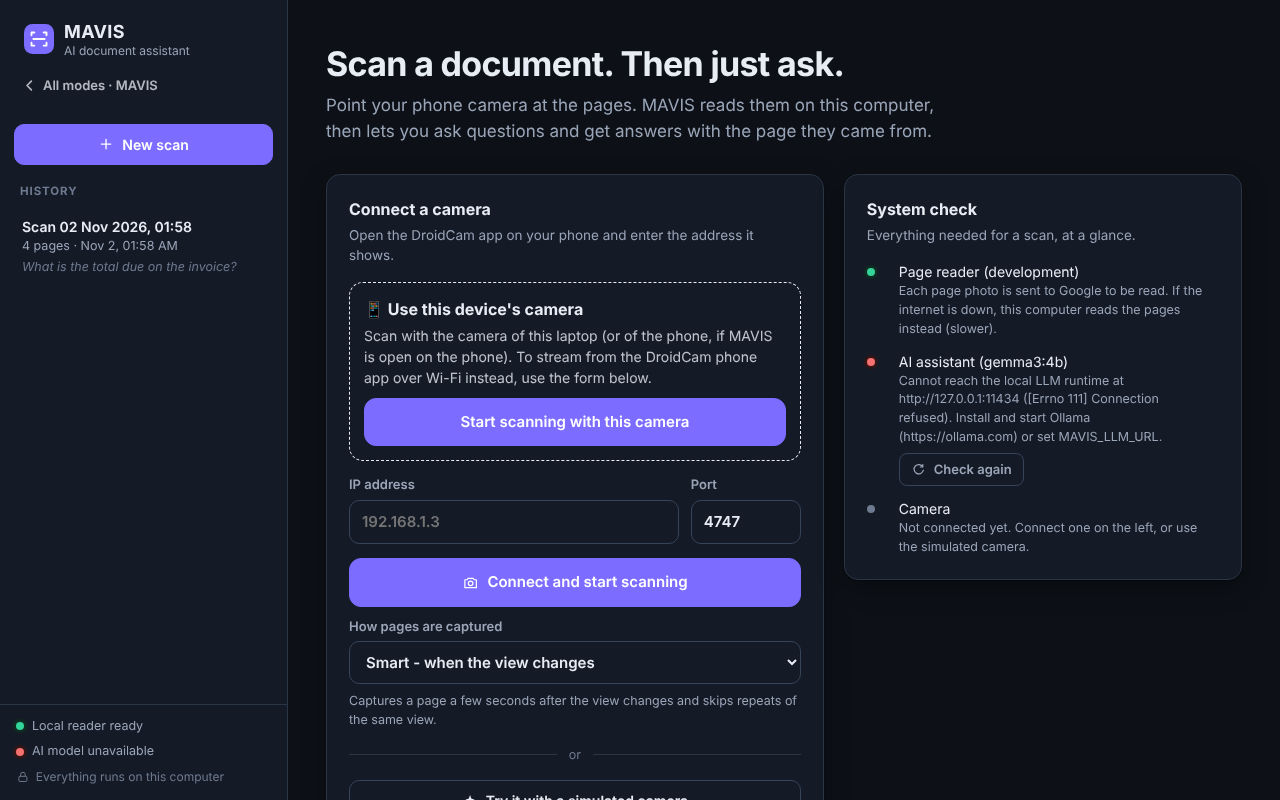
\includegraphics[width=0.56\textwidth]{f_ocr.png}
\caption{OCR + LLM start screen in the MAVIS theme: ``Use this device's camera'' or the DroidCam app by IP address and port}
\label{fig:ocr}
\end{figure}

\begin{figure}[H]
\centering
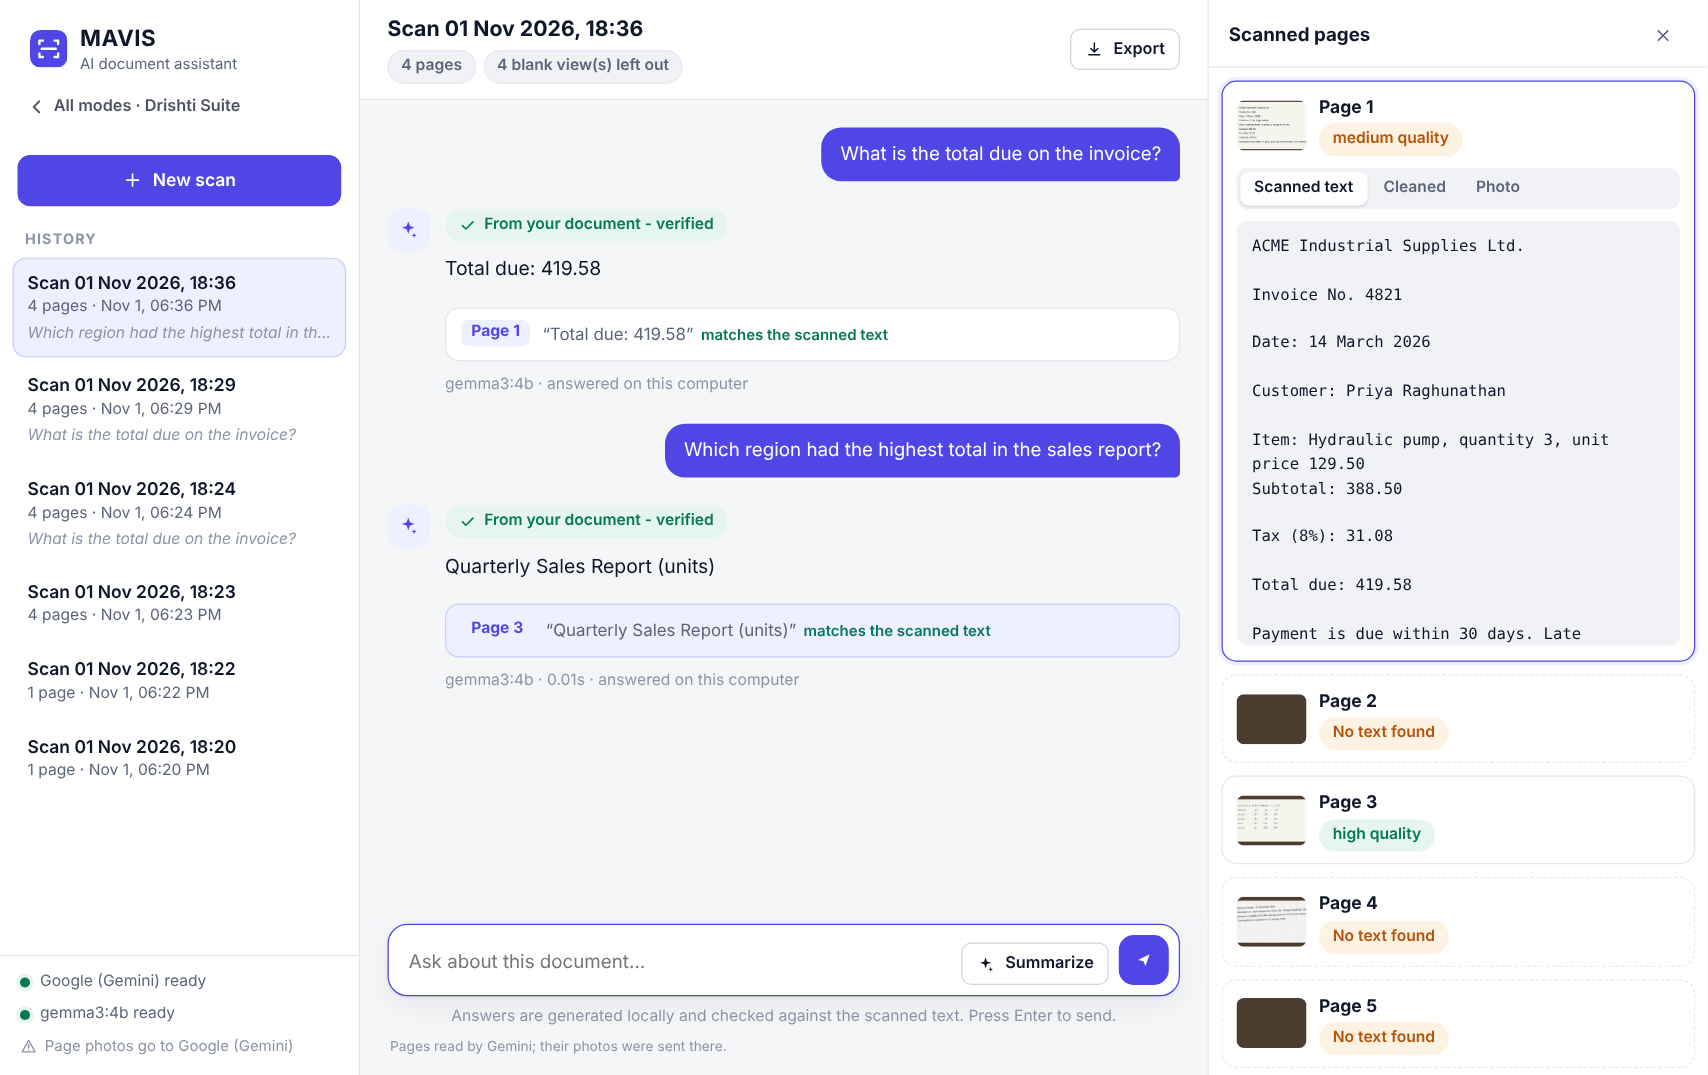
\includegraphics[width=0.56\textwidth]{mavis_answer.png}
\caption{Answers with page-cited quotes, each checked against the scanned text (``verified'')}
\label{fig:answer}
\end{figure}

\subsection{Live Translation}
\subsubsection{Recognition Quality (black book)}
On the same 300-file corpus (1105.8\,s of audio), the fixed-buffer baseline M1 and the streaming recogniser M2 used in MAVIS compare as in Table~\ref{tab:asr}. Streaming costs recognition quality---an expected and openly reported trade-off for showing text while the speaker is still talking---but the pipeline was robust: no failures, drops or ghost utterances over 509 decodes.

\begin{table}[H]
\centering
\caption{Speech recognition, M1 fixed buffer vs.\ M2 streaming, 300 files (black book)}
\label{tab:asr}
\small
\begin{tabular}{@{}lll@{}}
\toprule
\textbf{Metric} & \textbf{M1} & \textbf{M2 (streaming)} \\
\midrule
Corpus WER & 14.27\% & 24.30\% \\
Corpus CER & 7.62\% & 13.86\% \\
Detected utterances / ASR invocations & --- & 344 / 509 \\
ASR failures, queue drops, duplicates, ghost utterances & --- & 0, 0, 0, 0 \\
Files with all lifecycle checks passed & --- & 300 / 300 \\
Mean commitments per utterance; mean revisions & --- & 1.41; 0.148 \\
\bottomrule
\end{tabular}
\end{table}

\subsubsection{Translation Quality (black book)}
A standalone benchmark of the draft model opus-mt-en-hi on 10 utterances gave \textbf{BLEU 31.42} and \textbf{chrF 59.37}, with 713\,ms mean and 1443\,ms maximum model latency on CPU. This measures the draft model alone on complete sentences; final translations in MAVIS come from the larger NLLB-200 600M model.

\subsubsection{Live Sessions and Latency (black book)}
In live-microphone sessions with a scripted read, the word error rate against the script was 7.14\% on battery and 6.49\% on mains power, with one final per segment, no dropped frames and a clean shutdown. After four streaming defects found there were fixed, replays of the same recordings gave the latencies in Table~\ref{tab:trlat}. Start-up to listening took 13.7\,s on battery and 8.4\,s on mains; median ASR inference was 906\,ms and 487\,ms respectively; the worker peaked at about 1.6\,GB.

\begin{table}[H]
\centering
\caption{Latency of the final configuration, replayed live recordings (black book)}
\label{tab:trlat}
\small
\begin{tabularx}{\textwidth}{@{}p{2.8cm}XXX@{}}
\toprule
\textbf{Recording} & \textbf{First committed English (median, from speech onset)} & \textbf{First Hindi draft} & \textbf{Final Hindi after last word (median / max)} \\
\midrule
Battery & 4.31\,s & 5.57\,s & 2.34 / 3.10\,s \\
Mains power & 3.82\,s & 4.87\,s & 2.59 / 3.75\,s \\
\bottomrule
\end{tabularx}
\end{table}

\subsubsection{In MAVIS}
On the demonstration laptop the bridge selected the built-in microphone, the models loaded in \textbf{13.4\,s}, and spoken English produced Hindi subtitles over the live camera picture---for example, ``i love it'' was committed and translated by NLLB-200 into the natural Hindi equivalent (``I like this''). In the browser tests the subtitle page started by itself when opened by two fingers, showed drafts and then finals, and the EN line and transcript drawer worked.

\begin{figure}[H]
\centering
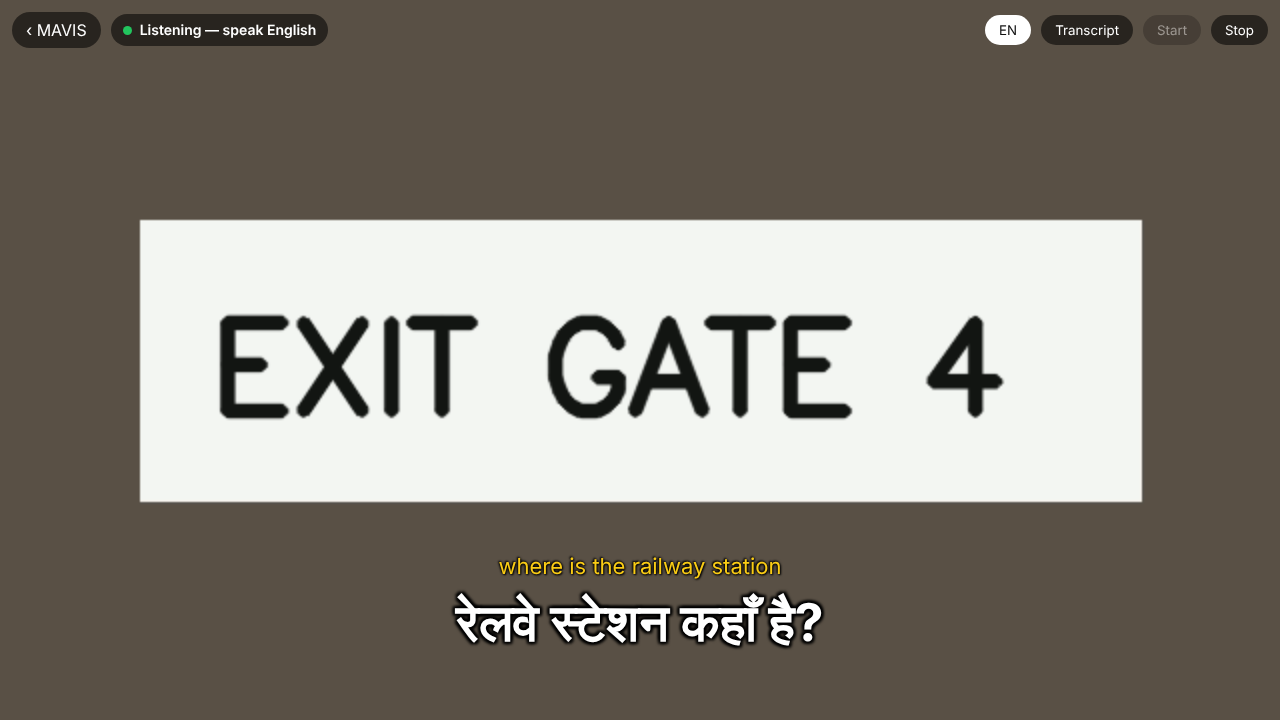
\includegraphics[width=0.56\textwidth]{f_translation.png}
\caption{Live Translation: Hindi subtitle over the laptop camera picture, with the optional English line}
\label{fig:translation}
\end{figure}

\subsection{Drishti}
\subsubsection{Hazard Scenarios (black book)}
Twelve realistic scenarios were run through Drishti's real hazard-scoring functions in the running application (Table~\ref{tab:hazard}). Every result matches the expected risk. Scenario~12 shows the intended behaviour of a deterministic safety layer: a truck very close and in the path is scored CRITICAL, but its distance confidence is LOW because its box is cut off by the frame edge.

\begin{table}[H]
\centering
\caption{Hazard-engine scenarios (black book)}
\label{tab:hazard}
\footnotesize
\begin{tabular}{@{}rllrlcl@{}}
\toprule
\textbf{\#} & \textbf{Scenario} & \textbf{Risk} & \textbf{Score} & \textbf{Proximity} & \textbf{In path} & \textbf{Dist. conf.} \\
\midrule
1 & Person close, directly ahead & CRITICAL & 13.50 & Very close & Yes & High \\
2 & Person far across the street & MEDIUM & 1.35 & Far & Yes & Medium \\
3 & Car approaching head-on, close & CRITICAL & 22.50 & Very close & Yes & High \\
4 & Car parked, far side & LOW & 0.90 & Far & No & Medium \\
5 & Bicycle passing, far left & MEDIUM & 1.80 & Medium & No & High \\
6 & Dog close, directly ahead & CRITICAL & 6.00 & Close & Yes & High \\
7 & Chair close, directly ahead & HIGH & 4.50 & Very close & Yes & High \\
8 & Bench, far side & LOW & 0.18 & Far & No & Medium \\
9 & Motorcycle close, to the side & HIGH & 4.80 & Close & No & High \\
10 & Bus far away, centred & MEDIUM & 2.25 & Far & Yes & Medium \\
11 & Stop sign nearby, to the side & LOW & 0.09 & Far & No & Medium \\
12 & Truck close, cut off by frame & CRITICAL & 22.50 & Very close & Yes & Low \\
\bottomrule
\end{tabular}
\end{table}

\subsubsection{Performance (black book)}
\begin{table}[H]
\centering
\caption{Measured component latencies in Drishti (black book)}
\label{tab:drperf}
\small
\begin{tabularx}{\textwidth}{@{}p{5.6cm}p{3.2cm}X@{}}
\toprule
\textbf{Component} & \textbf{Latency} & \textbf{Note} \\
\midrule
Local colour detection ($3\times3$) & 4.7--8.0\,ms & Pixel arithmetic \\
Hazard, tracking and priority engine & $\approx$0.03\,ms & Pure logic \\
Local OCR recognition (Tesseract.js) & 124--144\,ms & Clean text, 95\% confidence (used by Currency) \\
Local OCR worker load (first use) & 200--2350\,ms & One-time load \\
COCO-SSD detection & $\approx$4810\,ms & Headless, GPU-less test machine; not representative of laptops with WebGL \\
\bottomrule
\end{tabularx}
\end{table}

\subsubsection{In MAVIS}
When opened by three fingers, Drishti started its camera in Describe mode and took the first snapshot on its own (Figure~\ref{fig:ctldrishti}). The Read Text and Translate buttons were absent and all other modes and controls were present (Figure~\ref{fig:ctldrishti}). On the demonstration laptop Drishti's on-device models (2.1\,GB) were stored once during setup, and the team's live run used the laptop camera and microphone.



\subsection{The Integrated Product}
Figure~\ref{fig:launcher} shows the launcher with the four entries in the shared theme. On the demonstration laptop \texttt{run.bat} alone started Ollama, the hub and the browser, and in the team's live run the sequence---thumbs-up, choice, automatic start, open palm---worked with the built-in camera and microphone, while the DroidCam virtual devices were never picked by any module except when the user chose the phone stream in OCR + LLM.

\begin{figure}[H]
\centering
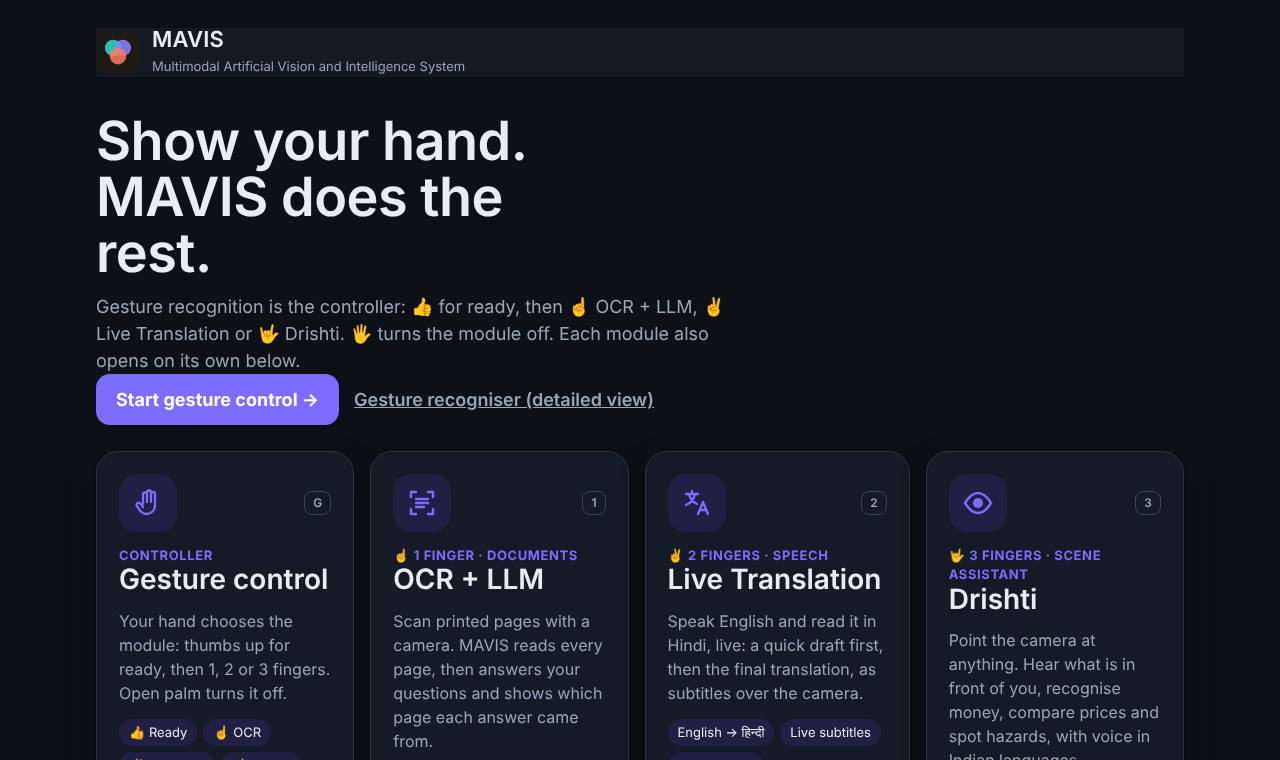
\includegraphics[width=0.56\textwidth]{f_launcher.png}
\caption{MAVIS launcher: gesture control and the three modules in one colour scheme}
\label{fig:launcher}
\end{figure}

\subsection{Comparative Analysis}
\label{sec:cmp}
\begin{table}[H]
\centering
\caption{Comparison of related work}
\label{tab:litcompare}
\footnotesize
\begin{tabularx}{\textwidth}{@{}p{3.7cm}*{6}{>{\centering\arraybackslash}X}@{}}
\toprule
\textbf{Work} & \textbf{Assistive focus} & \textbf{Reads documents} & \textbf{Verifiable answers} & \textbf{Speech translation} & \textbf{Gesture control} & \textbf{One product} \\
\midrule
VizWiz app \cite{bigham2010} & \cmark & Partial & \xmark\ (human) & \xmark & \xmark & \xmark \\
VizWiz dataset \cite{gurari2018} & \cmark & \xmark & \xmark & \xmark & \xmark & \xmark \\
SmolVLM \cite{marafioti2025} & \xmark & Partial & \xmark & \xmark & \xmark & \xmark \\
Gesture survey \cite{rautaray2015} & \xmark & \xmark & \xmark & \xmark & \cmark & \xmark \\
MediaPipe Hands \cite{zhang2020mediapipe} & \xmark & \xmark & \xmark & \xmark & Landmarks & \xmark \\
Tesseract, CRAFT, CRNN \cite{smith2007,baek2019,shi2017} & \xmark & \cmark & \xmark & \xmark & \xmark & \xmark \\
PP-OCR \cite{du2020ppocr} & \xmark & \cmark & \xmark & \xmark & \xmark & \xmark \\
DocVQA, RAG \cite{mathew2021,lewis2020} & \xmark & \cmark & Partial & \xmark & \xmark & \xmark \\
Whisper, Whisper-Streaming \cite{radford2023,machacek2023} & \xmark & \xmark & \xmark & ASR only & \xmark & \xmark \\
NLLB-200, OPUS-MT \cite{nllb2022,tiedemann2020} & \xmark & \xmark & \xmark & Text MT & \xmark & \xmark \\
Seeing AI, Be My AI \cite{seeingai,bemyeyes} & \cmark & \cmark & \xmark & \xmark & \xmark & \cmark\ (cloud) \\
\midrule
\textbf{MAVIS (this work)} & \cmark & \cmark & \cmark\ (quote check) & \cmark\ (live subtitles) & \cmark & \cmark\ (local) \\
\bottomrule
\end{tabularx}
\end{table}
Compared with the reviewed systems, MAVIS is the only one that puts document question answering with verified quotes, live speech translation and scene assistance behind one hands-free controller on a single laptop. It does not claim higher recognition, OCR or translation accuracy than its components; those remain as their authors measured them.

\subsection{Limitations}
Gesture end-to-end tests used video made from photographs of real hands, not a user study under varied lighting and distance. Streaming recognition costs about 10 percentage points of WER against the fixed-buffer baseline, the Hindi has had no native-speaker review, and the translation models take about 13\,s to load. Drishti's detection is slow without WebGL and its real-photo accuracy is not yet benchmarked. Only one module runs at a time by design.
%=====================================================================
\section{Conclusion and Further Work}
\subsection{Conclusion}
MAVIS turns four separately built systems into one assistive product controlled by the user's hand. The gesture recognition module became the controller: a thumbs-up arms it, one, two or three fingers open OCR + LLM, Live Translation or Drishti, the chosen module starts on its own, and an open palm turns it off. The OCR + LLM module reads pages from the laptop camera or the DroidCam phone app and answers with quotes that are checked against the scanned text; the translation module shows live Hindi subtitles of English speech over the camera picture, through its own host API in an isolated process and environment; and Drishti keeps its local-first scene assistance, hazard scoring and Indian-language voice, without the two modes that the dedicated modules now cover. Every module uses the laptop's own camera and microphone, the product has one colour scheme, and one batch file starts it.

No component's source was changed (314 byte-identical files) and every original test suite passes, with 21 new integration tests. The controller processed real hand photographs at 13.1\,ms per frame and opened an auto-started module in under 6\,s, while each module keeps the results its author measured.

\subsection{Further Work}
A user study with visually impaired users and Hindi-speaking listeners; keeping the translation worker warm so subtitles start within a second of the gesture; the planned M3 stability- and computation-aware translation scheduler with native-speaker evaluation; and labelled benchmark sets for Drishti and for document question answering.
\pagebreak

\addtocontents{toc}{\protect\setcounter{tocdepth}{1}}
\section{Research Paper}
Each member of the group is writing one research paper from the part of MAVIS they built. Papers~1 and~2 are complete drafts prepared for submission to ICONSIP 2027; Paper~3 is at the proposal stage and is yet to be drafted to a submittable level. Each paper will be attached here with its acceptance receipt and plagiarism report once submitted.

\subsection{Paper 1 --- Which Frames to Read? An Oracle-Based Benchmark of Causal Frame Selection for Video OCR}
\textbf{Lead author:} Varad Chipkar (OCR + LLM module); author names withheld in the draft for anonymous review.\\
\textbf{Status and target:} complete draft; to be submitted to ICONSIP 2027.

\textbf{Problem.} A camera reading aid cannot run OCR on every video frame, so it must choose which frames to read. Earlier frame-selection work scores page capture or frame quality, not the reading each selector actually commits compared with the best frame of the same video.

\textbf{Method.} A production-style capture loop and seven training-free causal selectors are replayed through a single-worker OCR queue on 207 public document videos (SmartDoc 2015, SmartDoc 2017 and WEZUT; 48,620 OCR'd frames). Each selector's reading is scored by its \emph{regret} against an exhaustive per-frame OCR oracle, with ground-truth, derived and proxy references kept apart. A separate measurement reports selector and OCR cost on one laptop.

\textbf{Key findings.} The production loop always committed to the opening frame, which was more than 0.10 worse than the best frame in 26 of 150 SmartDoc~2015 views, 15 of 24 SmartDoc~2017 views and all 20 WEZUT views. A selector that looks back about 4\,s and reads the sharpest frame had lower regret on every specification with 22--40\% fewer OCR calls; after multiplicity adjustment the gain was robust only on the single-page ground-truth dataset. Selectors cost milliseconds per frame against 2--4\,s per OCR call.

\textbf{Contributions.} A regret-based evaluation protocol for causal frame selection; a frozen public benchmark with traced provenance; evidence on design choices (sharpness, optical flow, start-up skip); and a single-machine CPU cost measurement.

\subsection{Paper 2 --- When to Re-translate: Workload--Freshness Trade-offs of MT Invocation Policies in a CPU-only Cascaded Speech-Translation Pipeline}
\textbf{Authors:} Yogita Aher, Varad Chipkar, Harshvardhan Deora, Suhas Kakade.\\
\textbf{Status and target:} complete draft; to be submitted to ICONSIP 2027.

\textbf{Problem.} A streaming translator that re-translates the growing transcript must decide how often to call the MT model: calling it on every stable update keeps the Hindi fresh but repeats work; waiting saves compute but delays new words. No examined work measures MT workload and freshness jointly across invocation policies on the same input.

\textbf{Method.} In the CPU-only English-to-Hindi cascade used by MAVIS (Faster-Whisper tiny with stable-prefix commitment and a frozen opus-mt-en-hi model), eight invocation conditions---eager, fixed thresholds of 8, 16 and 24 stable words, a threshold-plus-hold-deadline policy and three ablations---consume one frozen stable-ASR stream of 265 recordings and produce identical final translations. Every condition is timed with the same per-prefix MT service times in a modelled single-worker queue.

\textbf{Key findings.} Eager invocation re-translates 2.3 times the delivered words. Compared with it, the threshold-plus-deadline policy uses 0.79 times the MT compute (95\% CI 0.73--0.85) for 0.42\,s (0.37--0.47) more mean delay from a word becoming stable to its Hindi; at equal workload its delay matches the eager and fixed-threshold trade-off line, and its 2\,s deadline bounds policy hold, not total delay.

\textbf{Contributions.} A controlled replay design that isolates invocation decisions; a matched-service timing control; a workload--freshness characterisation of the three policy families; and sensitivity analyses.

\subsection{Paper 3 --- Harshvardhan Singh Deora (Drishti)}
\textbf{Title:} Local-First Hybrid Vision for Assistive Scene Understanding: Deterministic Hazard Scoring with On-Device Vision-Language Narration (working title).

\textbf{Research question.} Can a local-first hybrid architecture---on-device object detection, deterministic environment modelling and a small on-device vision-language model, with a cloud model used only as a fallback---improve reliability, latency and independence from paid APIs compared with the usual API-first design in which every camera frame is sent to a large cloud vision-language model, for assistive applications used by blind and visually impaired people?

\textbf{Approach.} Drishti's four-stage pipeline (Section~4.5) is the system under study. Safety-relevant judgements (hazard risk, path state, crossing view) are made only by the deterministic stage, never by the generative model, and every distance estimate carries a confidence tag. Three configurations are compared on the same images: \emph{Baseline-A}, cloud vision-language model only; \emph{Baseline-B}, local models only; and \emph{Hybrid}, Drishti's local-first pipeline with cloud fallback.

\textbf{Evaluation plan.} (1)~A labelled set of real indoor and outdoor photographs from Indian settings (people, vehicles, obstacles, currency, signs); (2)~object-detection precision and recall, agreement of hazard scores with human labels, and description quality rated by annotators; (3)~end-to-end latency on a mid-range laptop and phone, network calls per request, and behaviour without internet; (4)~the 12 hazard scenarios (Table~\ref{tab:hazard}) as a deterministic regression set. The comparison harness is built; the labelled photo set is being collected.

\textbf{Expected contribution.} Evidence that a meaningful share of assistive requests (object presence, hazards, path state, colour, currency) can be answered on the device with no API dependence and explainable output, with the cloud model reserved for open-ended questions.

\textbf{Target journal:} \tbd{to be decided}; the paper is yet to be drafted to a submittable level.

\vspace{1cm}
\section{Plagiarism Report}
\tbd{Attach the plagiarism report of this document here.}
\pagebreak

\renewcommand{\refname}{References}
{\footnotesize\setlength{\itemsep}{0pt}\setlength{\parskip}{0pt}
\begin{thebibliography}{99}
\setlength{\itemsep}{1pt}\setlength{\parsep}{0pt}
\addcontentsline{toc}{section}{References}

\bibitem{who2019} World Health Organization, \textit{World Report on Vision}, Geneva: WHO, 2019.

\bibitem{bourne2017} R. R. A. Bourne et al., ``Magnitude, temporal trends, and projections of the global prevalence of blindness and distance and near vision impairment: a systematic review and meta-analysis,'' \textit{The Lancet Global Health}, vol. 5, no. 9, pp. e888--e897, 2017.

\bibitem{seeingai} Microsoft, ``Seeing AI,'' https://www.seeingai.com (accessed 2026).

\bibitem{bemyeyes} Be My Eyes, ``Be My Eyes and Be My AI,'' https://www.bemyeyes.com (accessed 2026).

\bibitem{bigham2010} J. P. Bigham, C. Jayant, H. Ji, G. Little, A. Miller, R. C. Miller, R. Miller, A. Tatarowicz, B. White, S. White and T. Yeh, ``VizWiz: Nearly Real-Time Answers to Visual Questions,'' in \textit{Proc. 23rd ACM Symposium on User Interface Software and Technology (UIST)}, 2010, pp. 333--342.

\bibitem{gurari2018} D. Gurari, Q. Li, A. J. Stangl, A. Guo, C. Lin, K. Grauman, J. Luo and J. P. Bigham, ``VizWiz Grand Challenge: Answering Visual Questions from Blind People,'' in \textit{Proc. IEEE/CVF Conference on Computer Vision and Pattern Recognition (CVPR)}, 2018, pp. 3608--3617.

\bibitem{marafioti2025} A. Marafioti, O. Zohar, M. Farr\'{e}, M. Noyan, E. Bakouch, P. Cuenca et al., ``SmolVLM: Redefining Small and Efficient Multimodal Models,'' arXiv:2504.05299, 2025.

\bibitem{rautaray2015} S. S. Rautaray and A. Agrawal, ``Vision Based Hand Gesture Recognition for Human Computer Interaction: A Survey,'' \textit{Artificial Intelligence Review}, vol. 43, no. 1, pp. 1--54, 2015.

\bibitem{zhang2020mediapipe} F. Zhang, V. Bazarevsky, A. Vakunov, A. Tkachenka, G. Sung, C.-L. Chang and M. Grundmann, ``MediaPipe Hands: On-device Real-time Hand Tracking,'' CVPR Workshop on Computer Vision for Augmented and Virtual Reality, 2020; arXiv:2006.10214.

\bibitem{kapitanov2024} A. Kapitanov, K. Kvanchiani, A. Nagaev, R. Kraynov and A. Makhliarchuk, ``HaGRID -- HAnd Gesture Recognition Image Dataset,'' in \textit{Proc. IEEE/CVF Winter Conference on Applications of Computer Vision (WACV)}, 2024, pp. 4572--4581.

\bibitem{smith2007} R. Smith, ``An Overview of the Tesseract OCR Engine,'' in \textit{Proc. Ninth International Conference on Document Analysis and Recognition (ICDAR)}, IEEE, 2007, pp. 629--633.

\bibitem{baek2019} Y. Baek, B. Lee, D. Han, S. Yun and H. Lee, ``Character Region Awareness for Text Detection,'' in \textit{Proc. IEEE/CVF Conference on Computer Vision and Pattern Recognition (CVPR)}, 2019, pp. 9365--9374.

\bibitem{shi2017} B. Shi, X. Bai and C. Yao, ``An End-to-End Trainable Neural Network for Image-based Sequence Recognition and Its Application to Scene Text Recognition,'' \textit{IEEE Transactions on Pattern Analysis and Machine Intelligence}, vol. 39, no. 11, pp. 2298--2304, 2017.

\bibitem{du2020ppocr} Y. Du, C. Li, R. Guo, X. Yin, W. Liu, J. Zhou, Y. Bai, Z. Yu, Y. Yang, Q. Dang and H. Wang, ``PP-OCR: A Practical Ultra Lightweight OCR System,'' arXiv:2009.09941, 2020.

\bibitem{mathew2021} M. Mathew, D. Karatzas and C. V. Jawahar, ``DocVQA: A Dataset for VQA on Document Images,'' in \textit{Proc. IEEE/CVF Winter Conference on Applications of Computer Vision (WACV)}, 2021, pp. 2200--2209.

\bibitem{lewis2020} P. Lewis, E. Perez, A. Piktus, F. Petroni, V. Karpukhin, N. Goyal, H. K\"{u}ttler, M. Lewis, W. Yih, T. Rockt\"{a}schel, S. Riedel and D. Kiela, ``Retrieval-Augmented Generation for Knowledge-Intensive NLP Tasks,'' in \textit{Advances in Neural Information Processing Systems (NeurIPS)}, vol. 33, 2020.

\bibitem{ji2023} Z. Ji, N. Lee, R. Frieske, T. Yu, D. Su, Y. Xu, E. Ishii, Y. J. Bang, A. Madotto and P. Fung, ``Survey of Hallucination in Natural Language Generation,'' \textit{ACM Computing Surveys}, vol. 55, no. 12, art. 248, 2023.

\bibitem{liu2016ssd} W. Liu, D. Anguelov, D. Erhan, C. Szegedy, S. Reed, C.-Y. Fu and A. C. Berg, ``SSD: Single Shot MultiBox Detector,'' in \textit{Proc. European Conference on Computer Vision (ECCV)}, 2016, pp. 21--37.

\bibitem{sandler2018} M. Sandler, A. Howard, M. Zhu, A. Zhmoginov and L.-C. Chen, ``MobileNetV2: Inverted Residuals and Linear Bottlenecks,'' in \textit{Proc. IEEE/CVF Conference on Computer Vision and Pattern Recognition (CVPR)}, 2018, pp. 4510--4520.

\bibitem{gemma3} Gemma Team, Google DeepMind, ``Gemma 3 Technical Report,'' arXiv:2503.19786, 2025.

\bibitem{rfc6455} I. Fette and A. Melnikov, ``The WebSocket Protocol,'' RFC 6455, IETF, 2011.

\bibitem{w3cmediacapture} W3C, ``Media Capture and Streams,'' W3C Candidate Recommendation, https://www.w3.org/TR/mediacapture-streams/.

\bibitem{w3csecure} W3C, ``Secure Contexts,'' W3C Candidate Recommendation, https://www.w3.org/TR/secure-contexts/.

\bibitem{mediapipe_repo} Google, ``MediaPipe,'' https://github.com/google-ai-edge/mediapipe.

\bibitem{rapidocr} RapidAI, ``RapidOCR,'' https://github.com/RapidAI/RapidOCR.


\bibitem{radford2023} A. Radford, J. W. Kim, T. Xu, G. Brockman, C. McLeavey and I. Sutskever, ``Robust Speech Recognition via Large-Scale Weak Supervision,'' in \textit{Proc. 40th International Conference on Machine Learning (ICML)}, PMLR 202, 2023, pp. 28492--28518.

\bibitem{machacek2023} D. Mach\'{a}\v{c}ek, R. Dabre and O. Bojar, ``Turning Whisper into Real-Time Transcription System,'' in \textit{Proc. IJCNLP-AACL 2023: System Demonstrations}, 2023, pp. 17--24.

\bibitem{papi2025} S. Papi, P. Pol\'{a}k, D. Mach\'{a}\v{c}ek and O. Bojar, ``How `Real' is Your Real-Time Simultaneous Speech-to-Text Translation System?,'' \textit{Transactions of the Association for Computational Linguistics}, vol. 13, 2025.

\bibitem{nllb2022} NLLB Team, M. R. Costa-juss\`{a} et al., ``No Language Left Behind: Scaling Human-Centered Machine Translation,'' arXiv:2207.04672, 2022; \textit{Nature}, vol. 630, pp. 841--846, 2024.

\bibitem{tiedemann2020} J. Tiedemann and S. Thottingal, ``OPUS-MT --- Building Open Translation Services for the World,'' in \textit{Proc. 22nd Annual Conference of the European Association for Machine Translation (EAMT)}, 2020, pp. 479--480.

\bibitem{silero} Silero Team, ``Silero VAD: pre-trained enterprise-grade Voice Activity Detector,'' https://github.com/snakers4/silero-vad (accessed 2026).

\end{thebibliography}

}
\end{document}
